\chapter{Description and Features List}

\section{ToM+ Feature Highlights}

ToM+ has many functions and can be constantly updated along with the firmware
development. In the next few paragraphs I will give you a brief introduction of its
features, to give you an idea of the type of product that I will explain later in the manual.

\subsection{A new Twizy dashboard}

Since the dashboard of our Twizy includes some values only, like the speed and the
remaining kilometers, I decided to develop this cool display, that will show much
more data, reading them directly from the Twizy CAN bus, using the OBD connector
in the left glove box. ToM will just “sniff” the values sent out by the Twizy and then
 show them on the LCD display, allowing many other features. ToM has a tiny
but powerful memory that is able to store some of these values while driving to give
you a trip history. The capability of it to store some values, makes it possible to
save your configurations and customizations on ToM, even after a firmware update.

\begin{figure}[H]
    \centering
    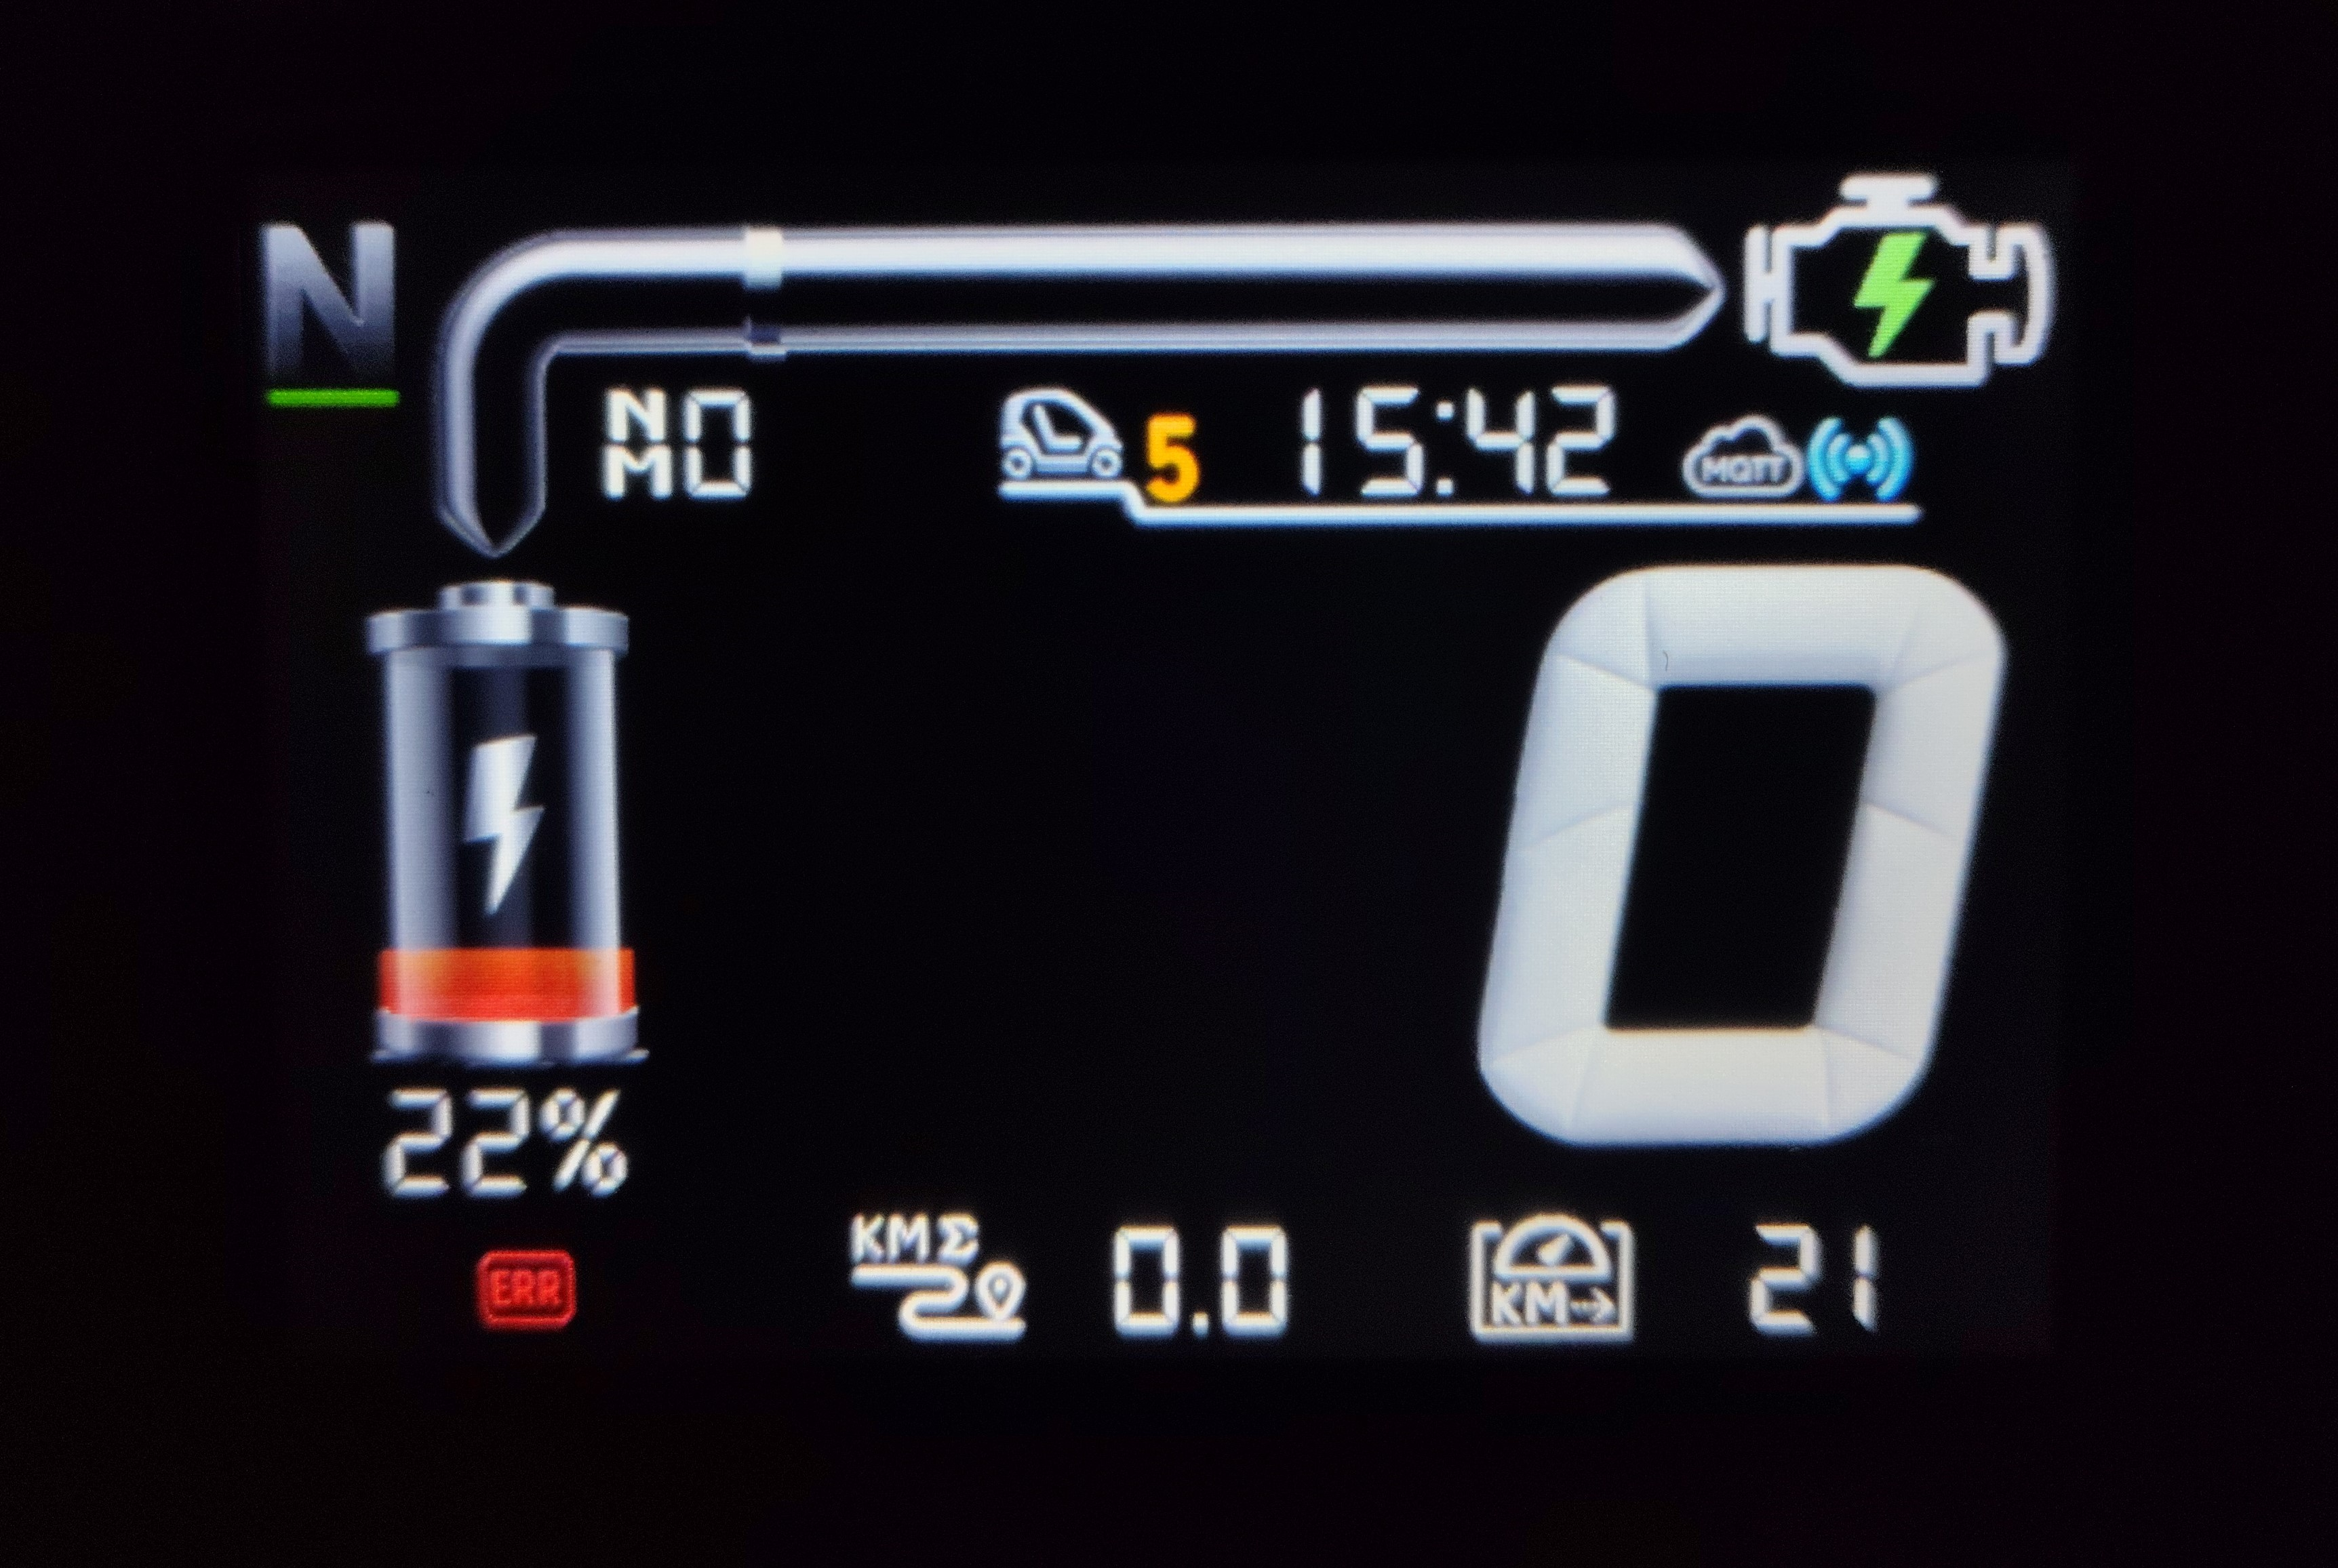
\includegraphics[width=0.8\textwidth]{figures/dashboard.jpg}
    \caption{Dashboard of the ToM+}
\end{figure}

It tries to keep the same style of the original Twizy dashboard, but with a more modern and
3D look.
As the original one you have the battery, gear, the remaining kilometers, the speed and the time.
But I added the exact \textbf{battery percentage}, the engine torque, some status icons, trip information and a lot of other stuff that you can configure as you wish and we will see in detail later.

The main page is customizable and you can choose what to show on it, as well as the other pages that you can scroll through using the button you can mount on the wiper stalk.
The general look of the other pages is shown in the image, with one value in the foreground and the others in the left side. In the bottom
you can change the shown page by tapping its icon.

\begin{figure}[H]
    \centering
    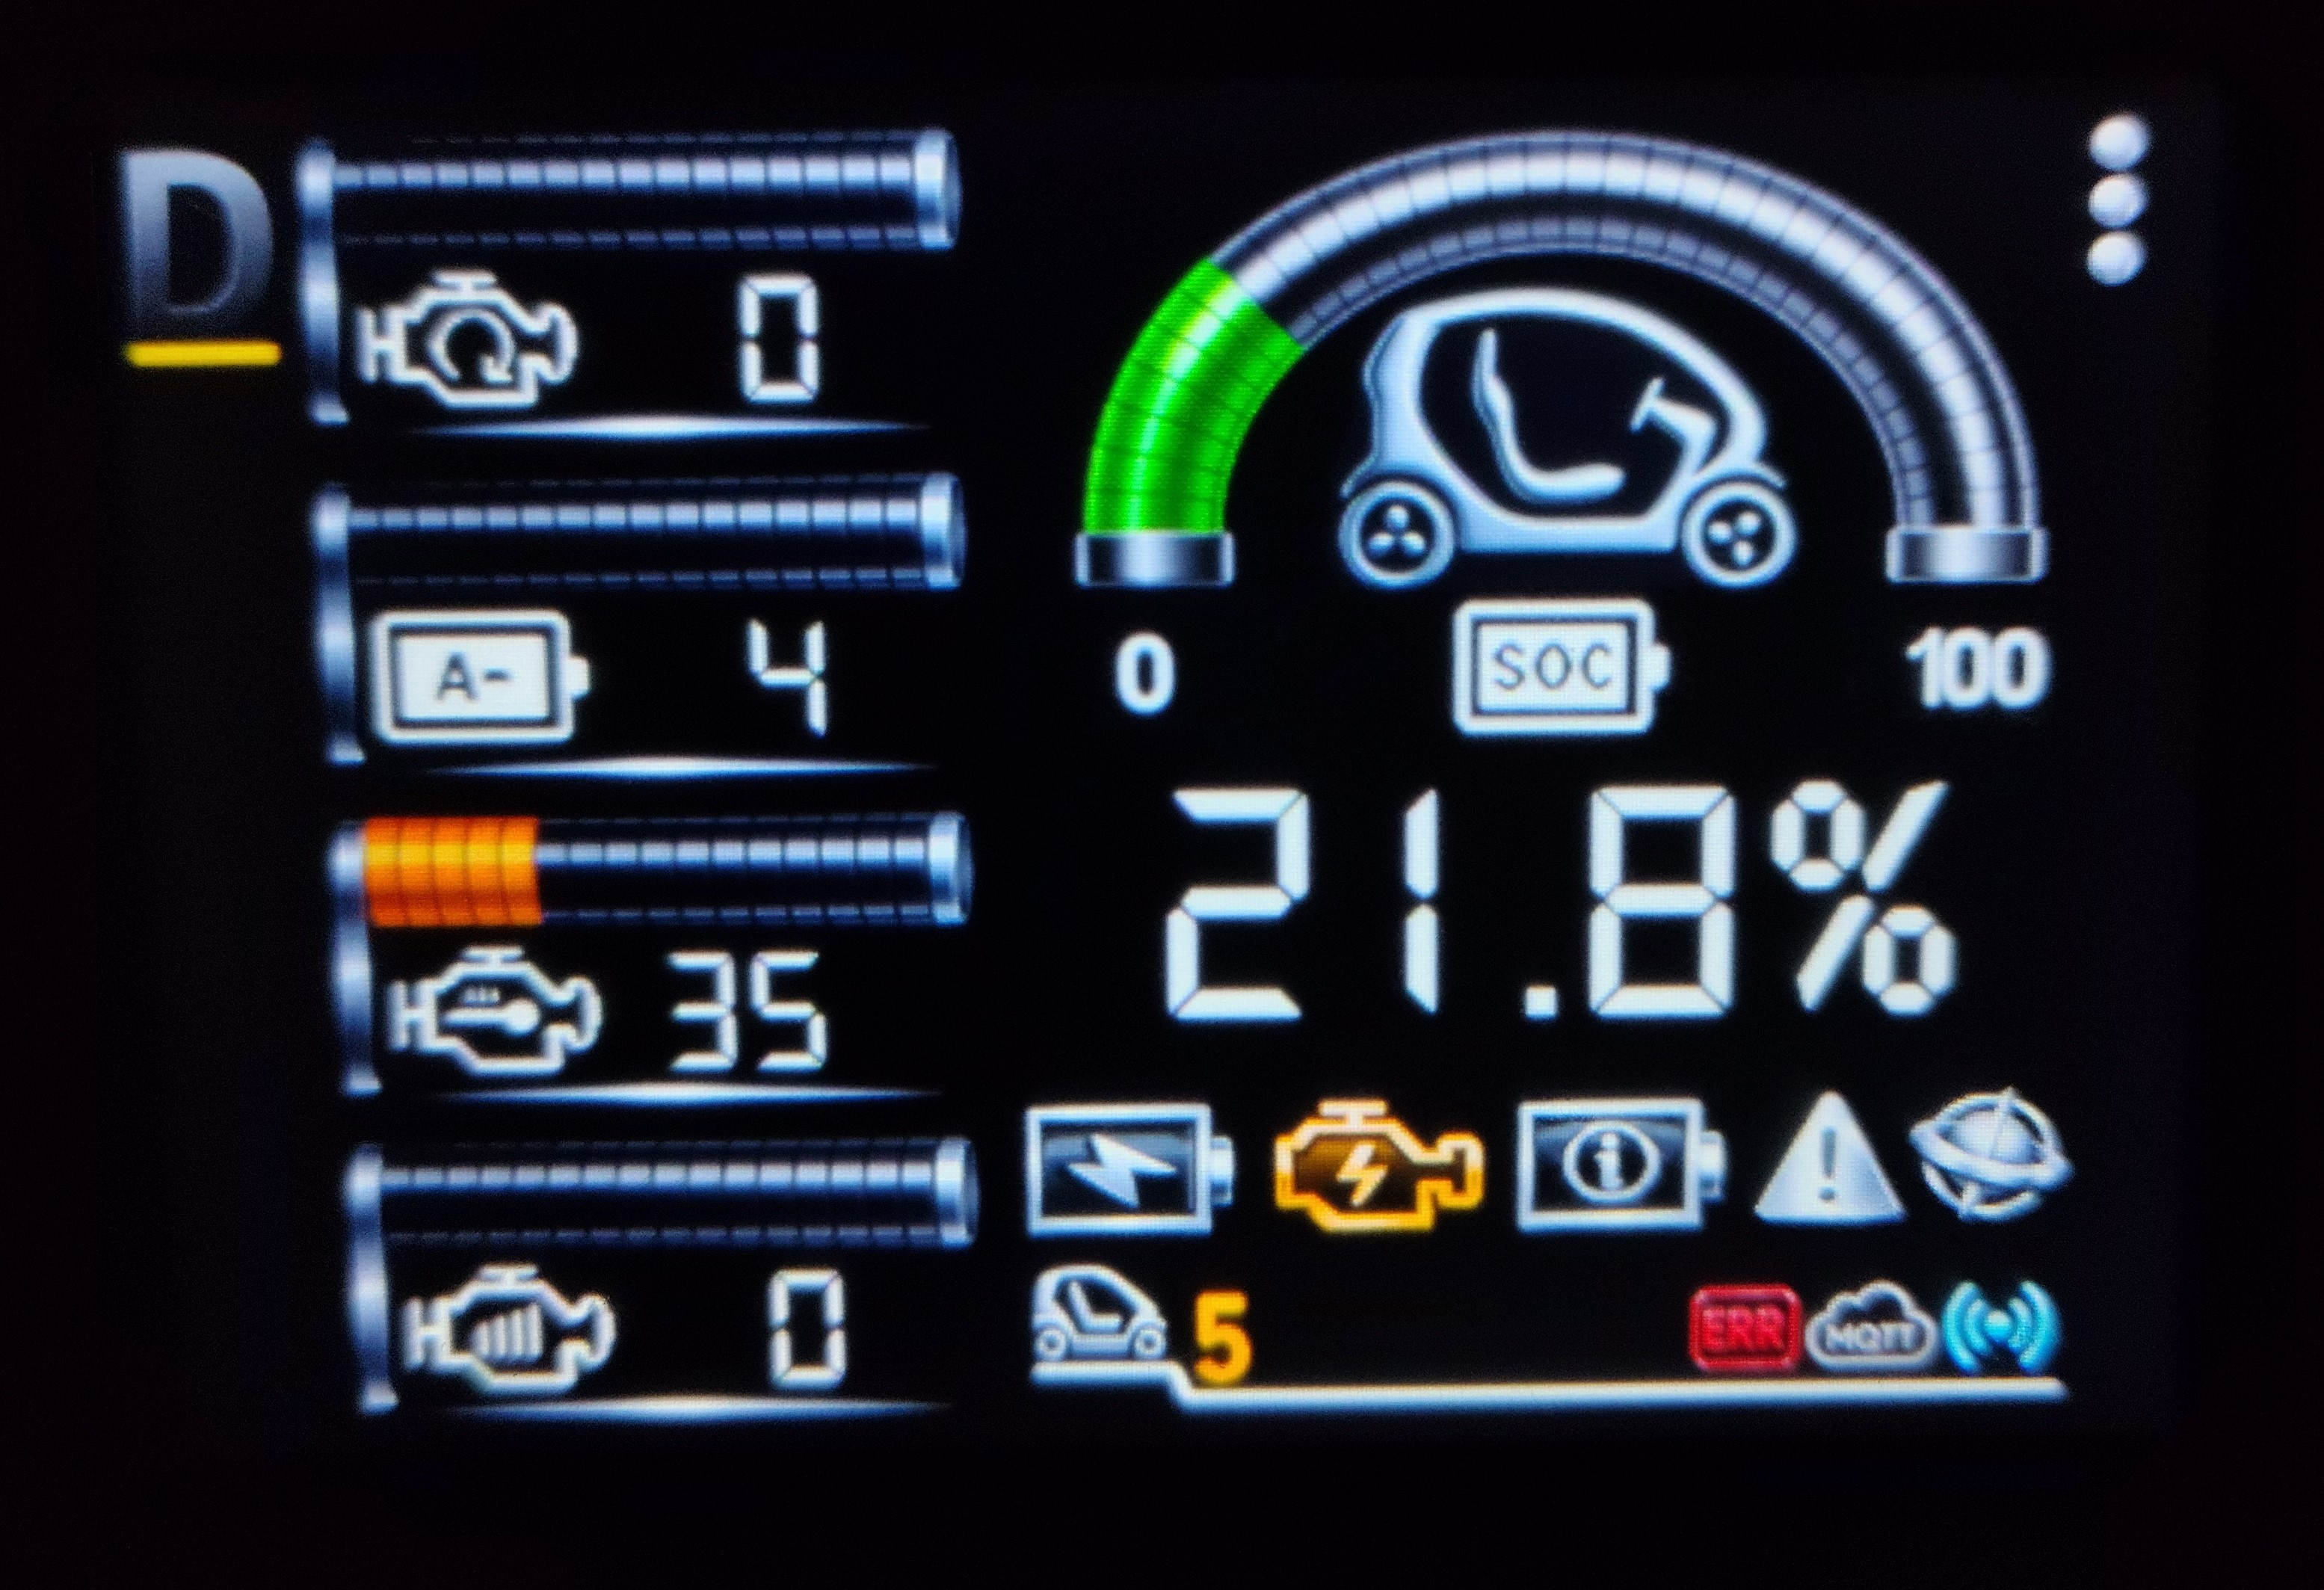
\includegraphics[width=0.8\textwidth]{figures/engine_page.jpg}
    \caption{Engine page of the ToM+}
\end{figure}

\subsection{WiFi connectivity}

The ESP32 board contained in the black box have the capability to connect to a WiFi
network access point. Once ToM+ is connected you can do plenty of things. For
instance, this device can be used to transfer data from your Twizy to your personal \textbf{MQTT}
broker, where you can use these values to embed your car in your home automation IoT system. 

This is not the only feature related to the Wi-Fi capability that ToM+ has. It's able to be 
an access point as well with its SSID and password, creating a private network with no 
Internet connection. In this way you can safely connect, \textbf{accepting to keep the connection}
 profile active even if it doesn't provide any Internet connection (it usually appears with a
notify in Android phones 10 seconds after the first connection) and then perform your
additional configurations on some web server pages hosted by ToM+ itself. Just type
in your favorite browser ToM static private IPv4 (\textbf{\textit{192.188.1.188}}) and enjoy!

\begin{figure}[H]
    \centering
    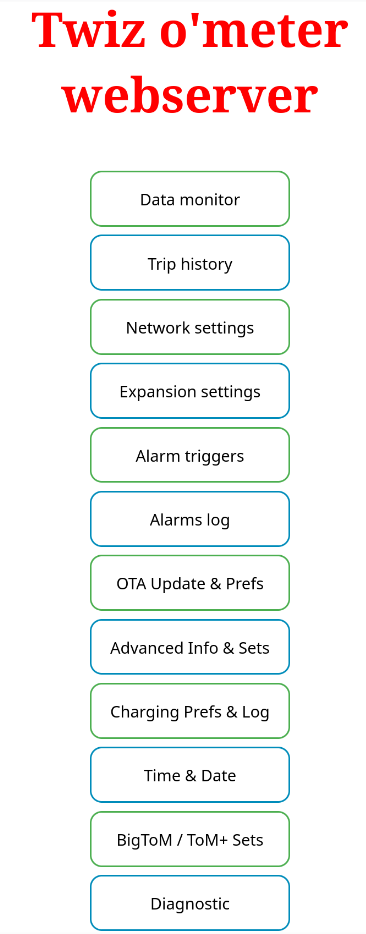
\includegraphics[
        width=\textwidth,
        height=0.75\textheight,
        keepaspectratio
    ]{figures/landing_page.png}
    \caption{Web server landing page}
\end{figure}

As you can see in this new version of ToM, the web server is much more complete and user friendly. You can easily navigate through the pages and configure your device as you wish. The web server is also responsive, so you can use it on your smartphone or tablet as well.

\subsection{ToM phone application}

Along with LCD and black box firmware updates, a minimal Android application is
kept updated as well and will allow you to monitor your Twizy real-time data using
your smart phone. 

The layout tries to emulate the ToM original graphical interface and relies on \textbf{MQTT} protocol to share
and transfer values from ToM+ to the application, so you will need to configure it both
on the app and on ToM+ MQTT page, swapping the IN and OUT topics. The app is
distributed with an \textbf{APK} file, a packaged installer for Android applications which
allow you to mount this app even without an Internet connection.

You may need to enable “install apps from unknown sources” flag in your phone settings to open such a file
extension \textit{(.apk)}. At first start you may notice a pop-up saying that this application
was created for an older version of Android if you have a newer phone: just say OK
and ignore it (it will work fine). Some preview of the charging and settings page of the app:

\begin{figure}[H]
    \centering
    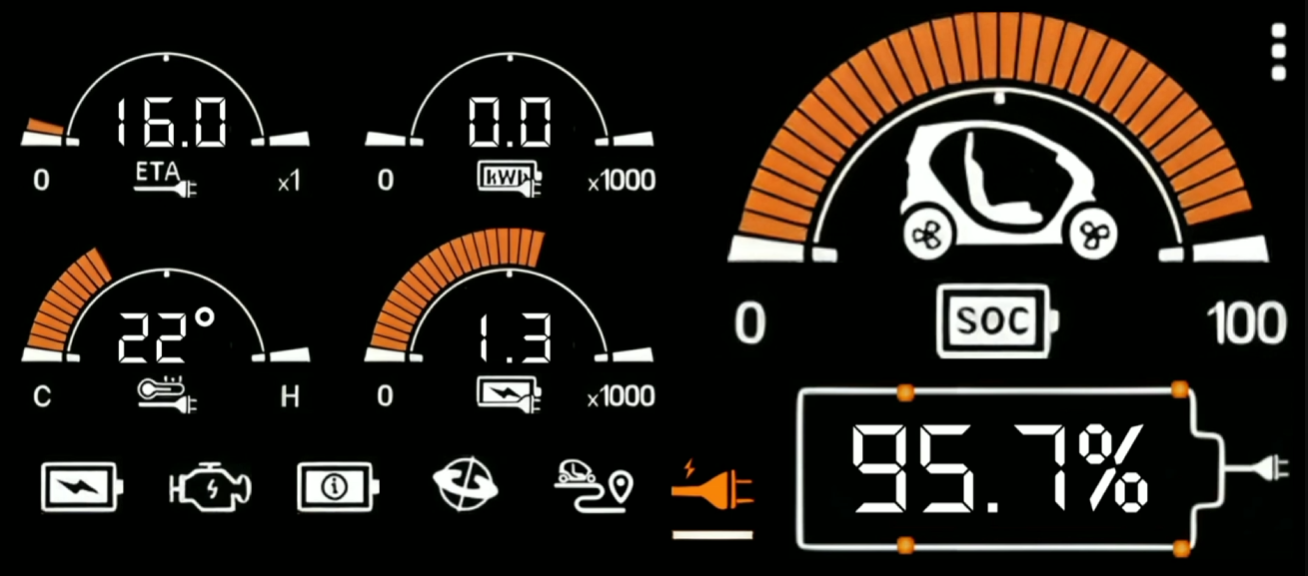
\includegraphics[width=0.8\textwidth]{figures/tom_app_charging.png}
    \caption{Charging page of the ToM+ Android app}
\end{figure}

\begin{figure}[H]
    \centering
    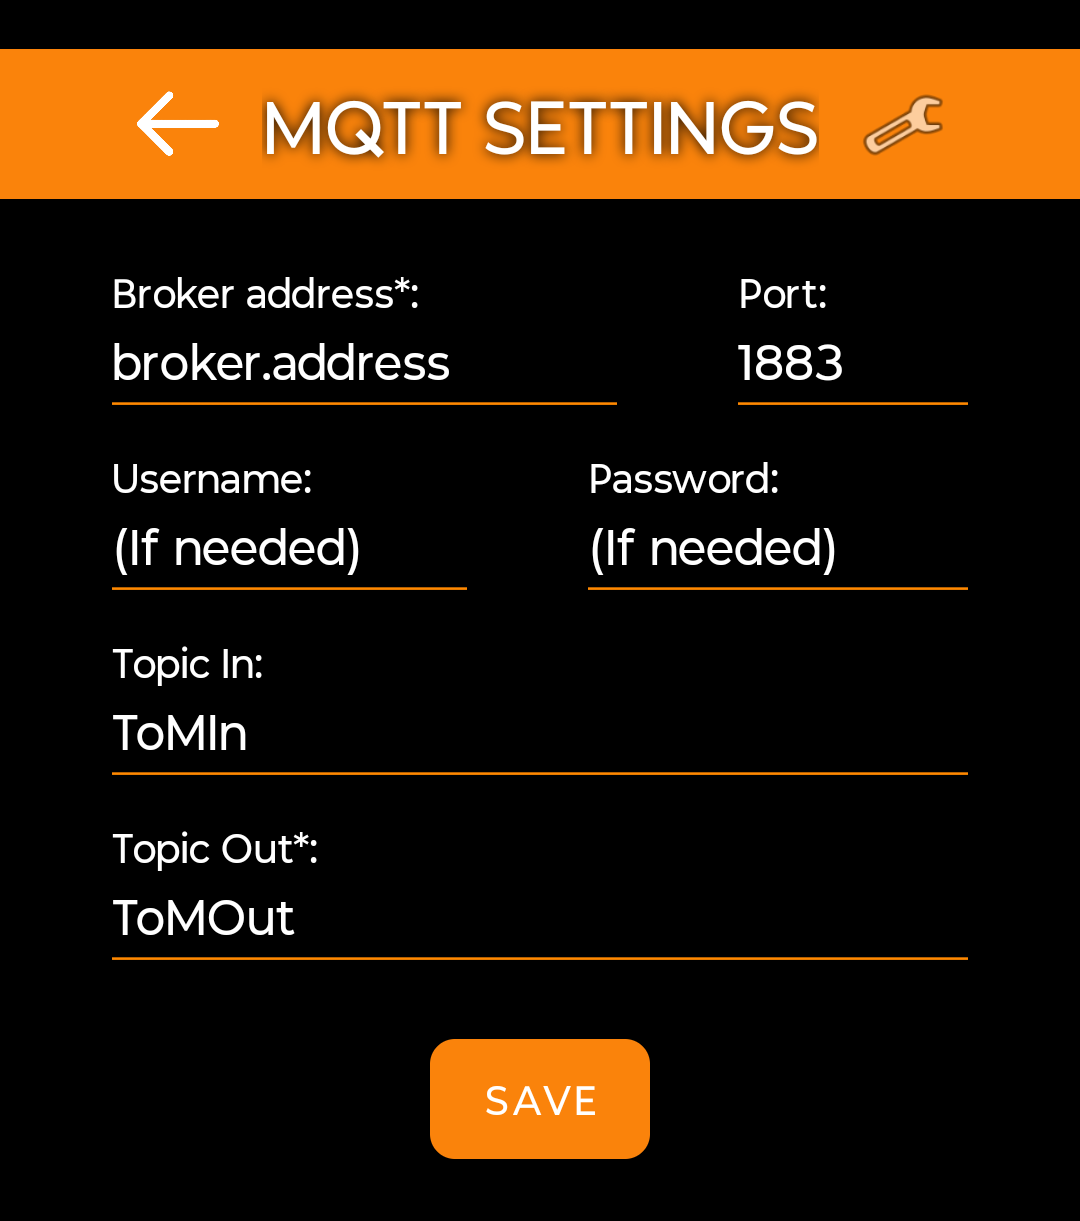
\includegraphics[width=0.65\textwidth]{figures/tom_app_settings.png}
    \caption{Settings page of the ToM+ Android app}
\end{figure}

\subsection{Brief consumption overview}

ToM will use the 12V battery power supply, taking it directly from the OBD connector and
won't consume much, as shown in the progressive measures down below.

\begin{figure}[H]
    \centering
    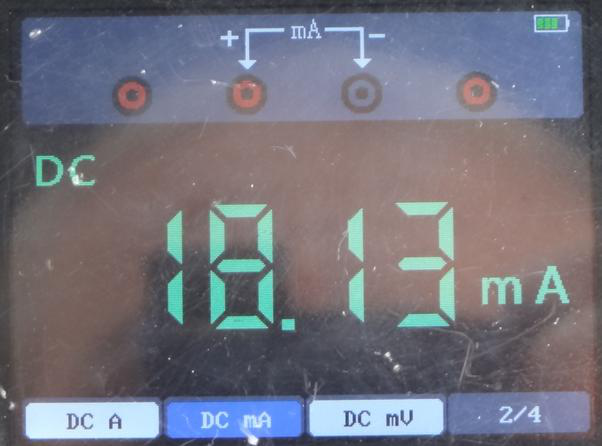
\includegraphics[width=0.65\textwidth]{figures/consumption_off.png}
    \caption{Consumption when Twizy is OFF}
\end{figure}

When the motherboard is active and the display is turned on, it consumes about 90 mA. If the WiFi is turned on as well, the power consumption is around the one shown below (maybe a little more due to the last updates that introduced the 3D graphic).

\begin{figure}[H]
    \centering
    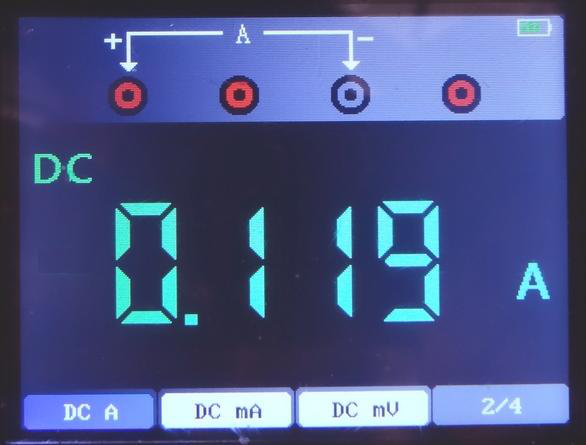
\includegraphics[width=0.65\textwidth]{figures/consumption_on_wifi.png}
    \caption{Consumption when ToM+ is ON with WiFi}
\end{figure}

When Twizy is OFF, the black box will go to sleep mode and will consume 18 mA.
In addition, the touch capability will allow you to interact much more easily with the
device and its LCD display. Since it uses a resistive touch technology, you can use  your
 fingers or a small hard plastic stylus pen to press the buttons. It's not as powerful as
  capacitive touch screen dashboards but once you have tried it, you can't do without, 
  trust me!

\clearpage

\section{Provided ToM+ Kit}

When ToM+ is shipped, it is usually packaged in a brown box to protect internal boards
and sensors from bumps during the travel. In this newer version, no more long cables are needed, just a shorter one connected to the internal ToM+ motherboard, enclosed in a small black plastic
container that I usually call “black box”. Of course, along with it, the resistive LCD touch display is provided, where you can view and configure all the stuff.
No more screws or tape needed! Just an easy clip on display that fits directly on top of the original dashboard.

\begin{figure}[H]
    \centering
    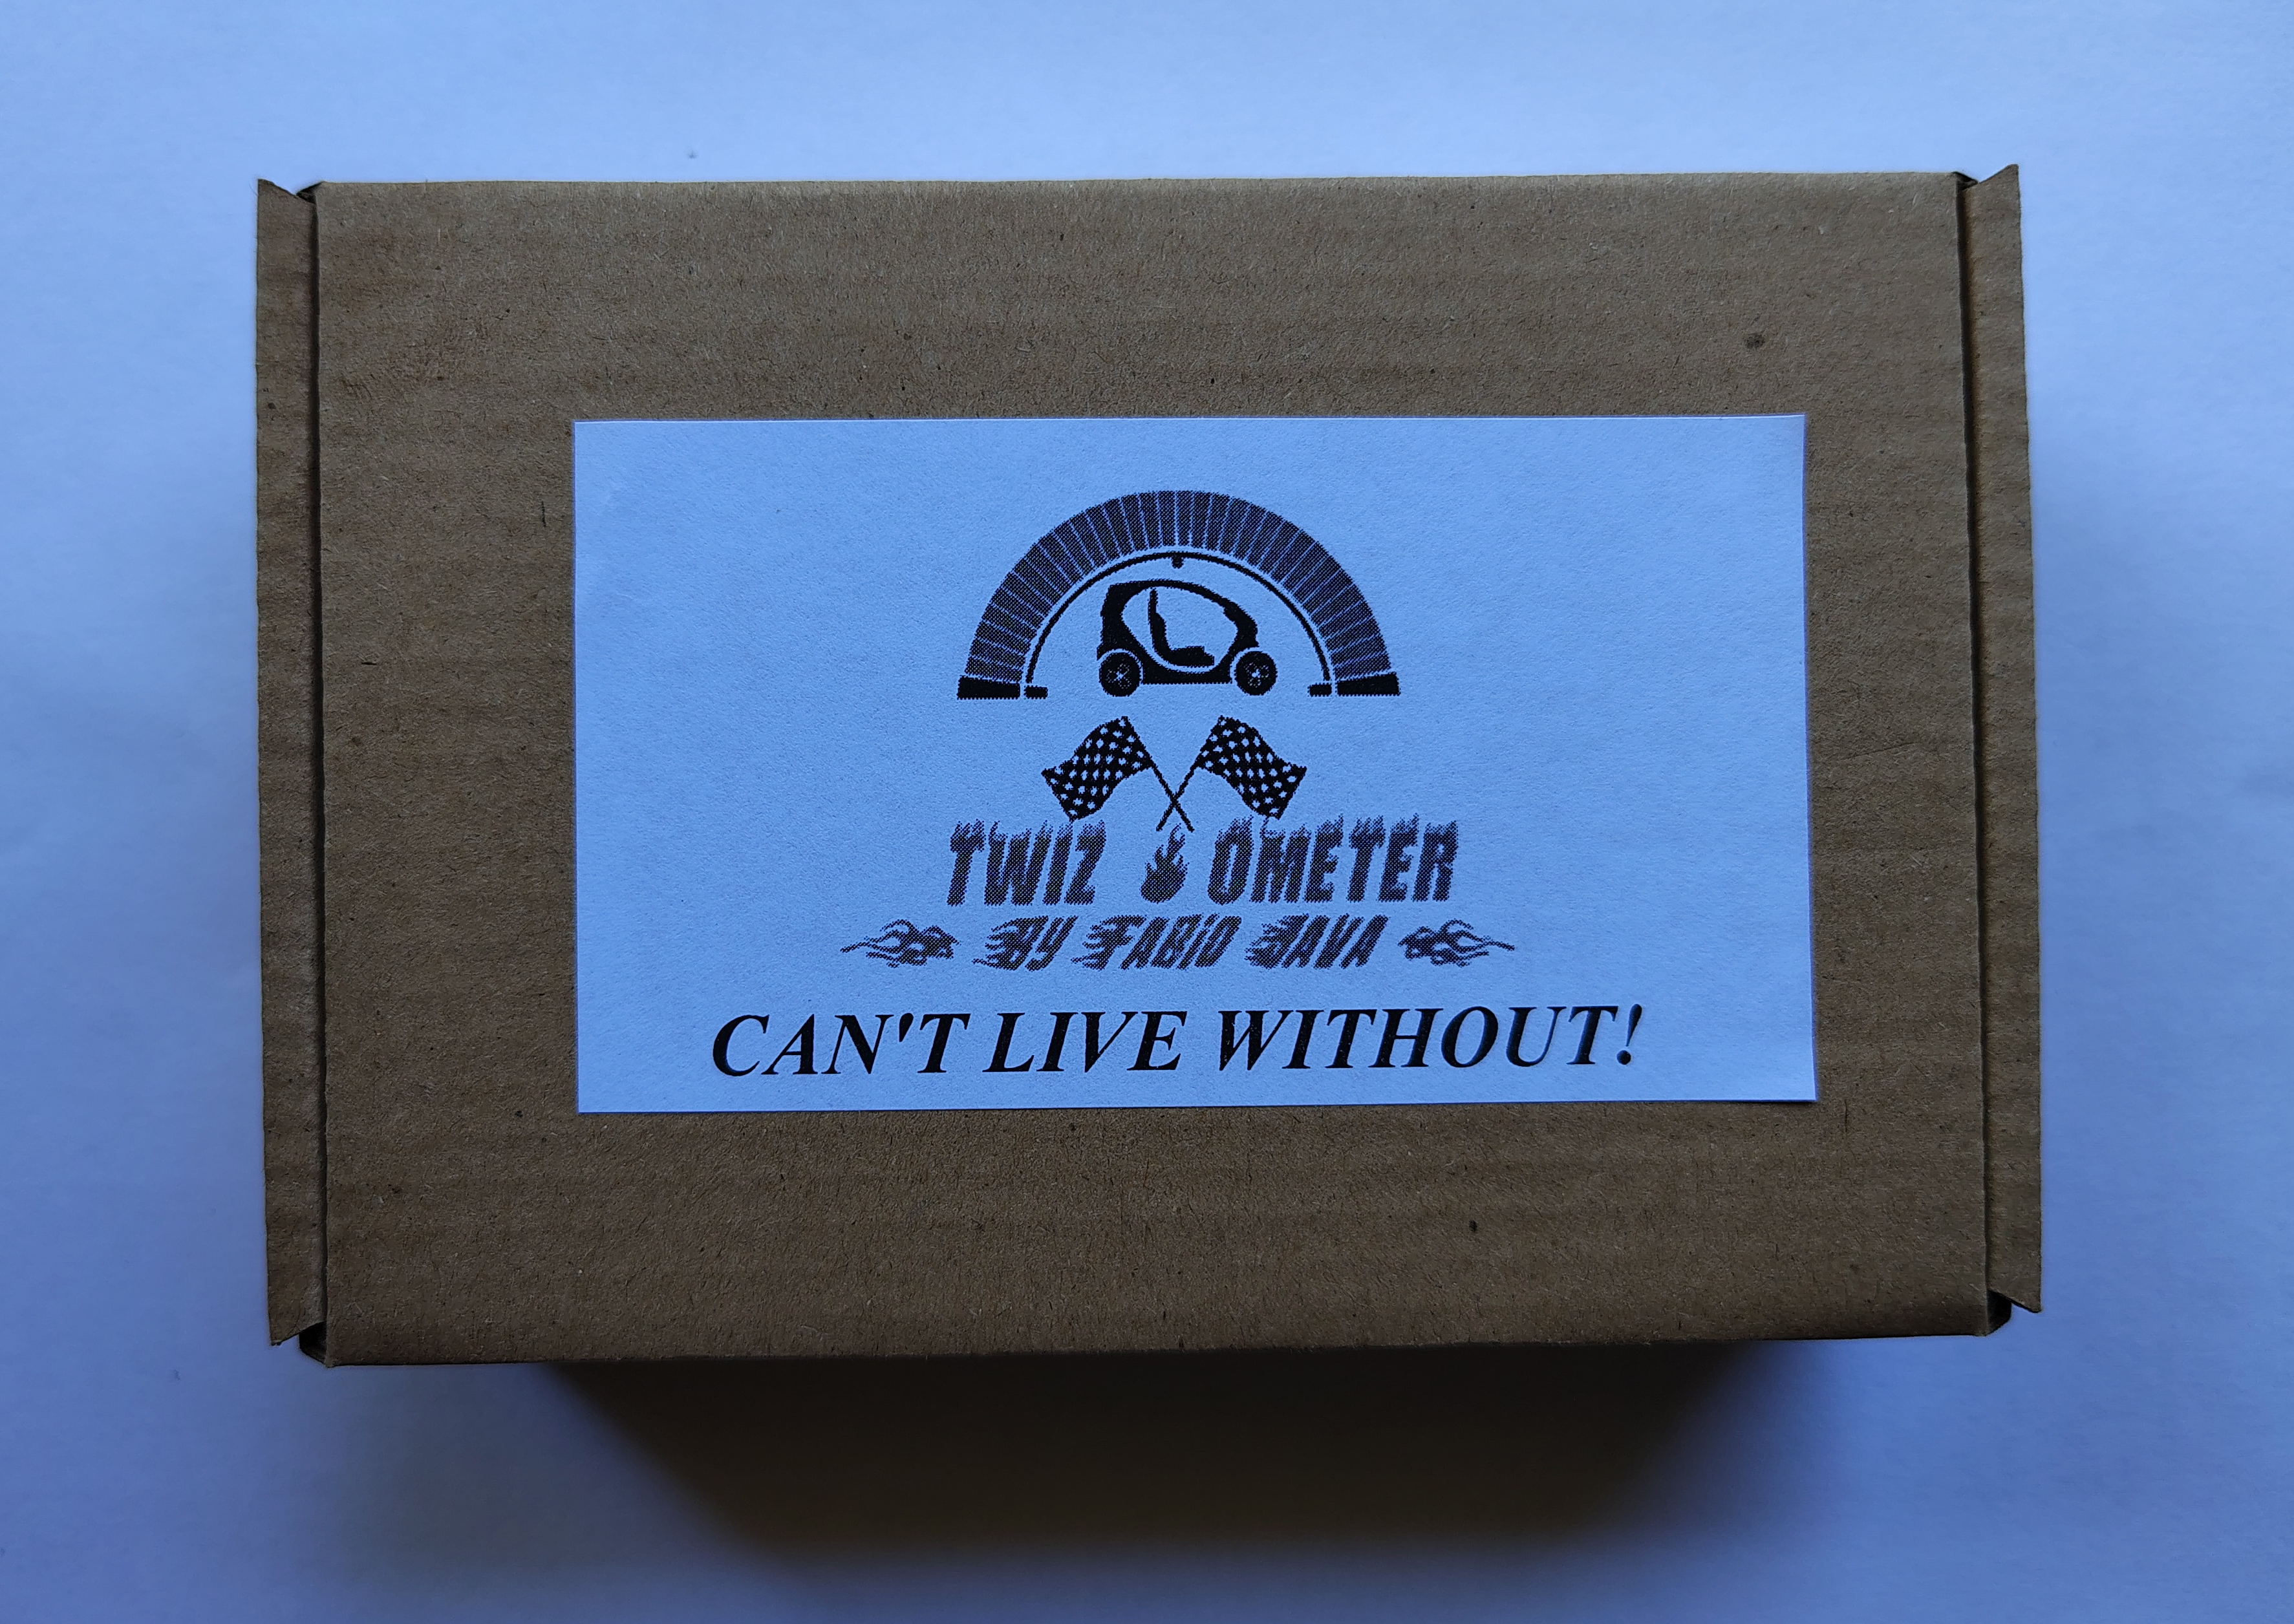
\includegraphics[width=0.8\textwidth]{figures/box.png}
    \caption{Provided ToM+ kit}
\end{figure}

\subsection{The Black Box}

The black box is the motherboard of ToM+ and contains most of the components needed
for the system to operate. It provides:
\begin{itemize}
    \item An external connector for the LCD display;
    \item An expansion connector with power and GPIO pins;
    \item An on-board OBD female port for the Twizy CAN bus;
    \item A microUSB port for firmware updates;
    \item A female connector for the button on the wiper stalk.
    \item ON/OFF ToM+ power switch
\end{itemize}

\begin{figure}[H]
    \centering
    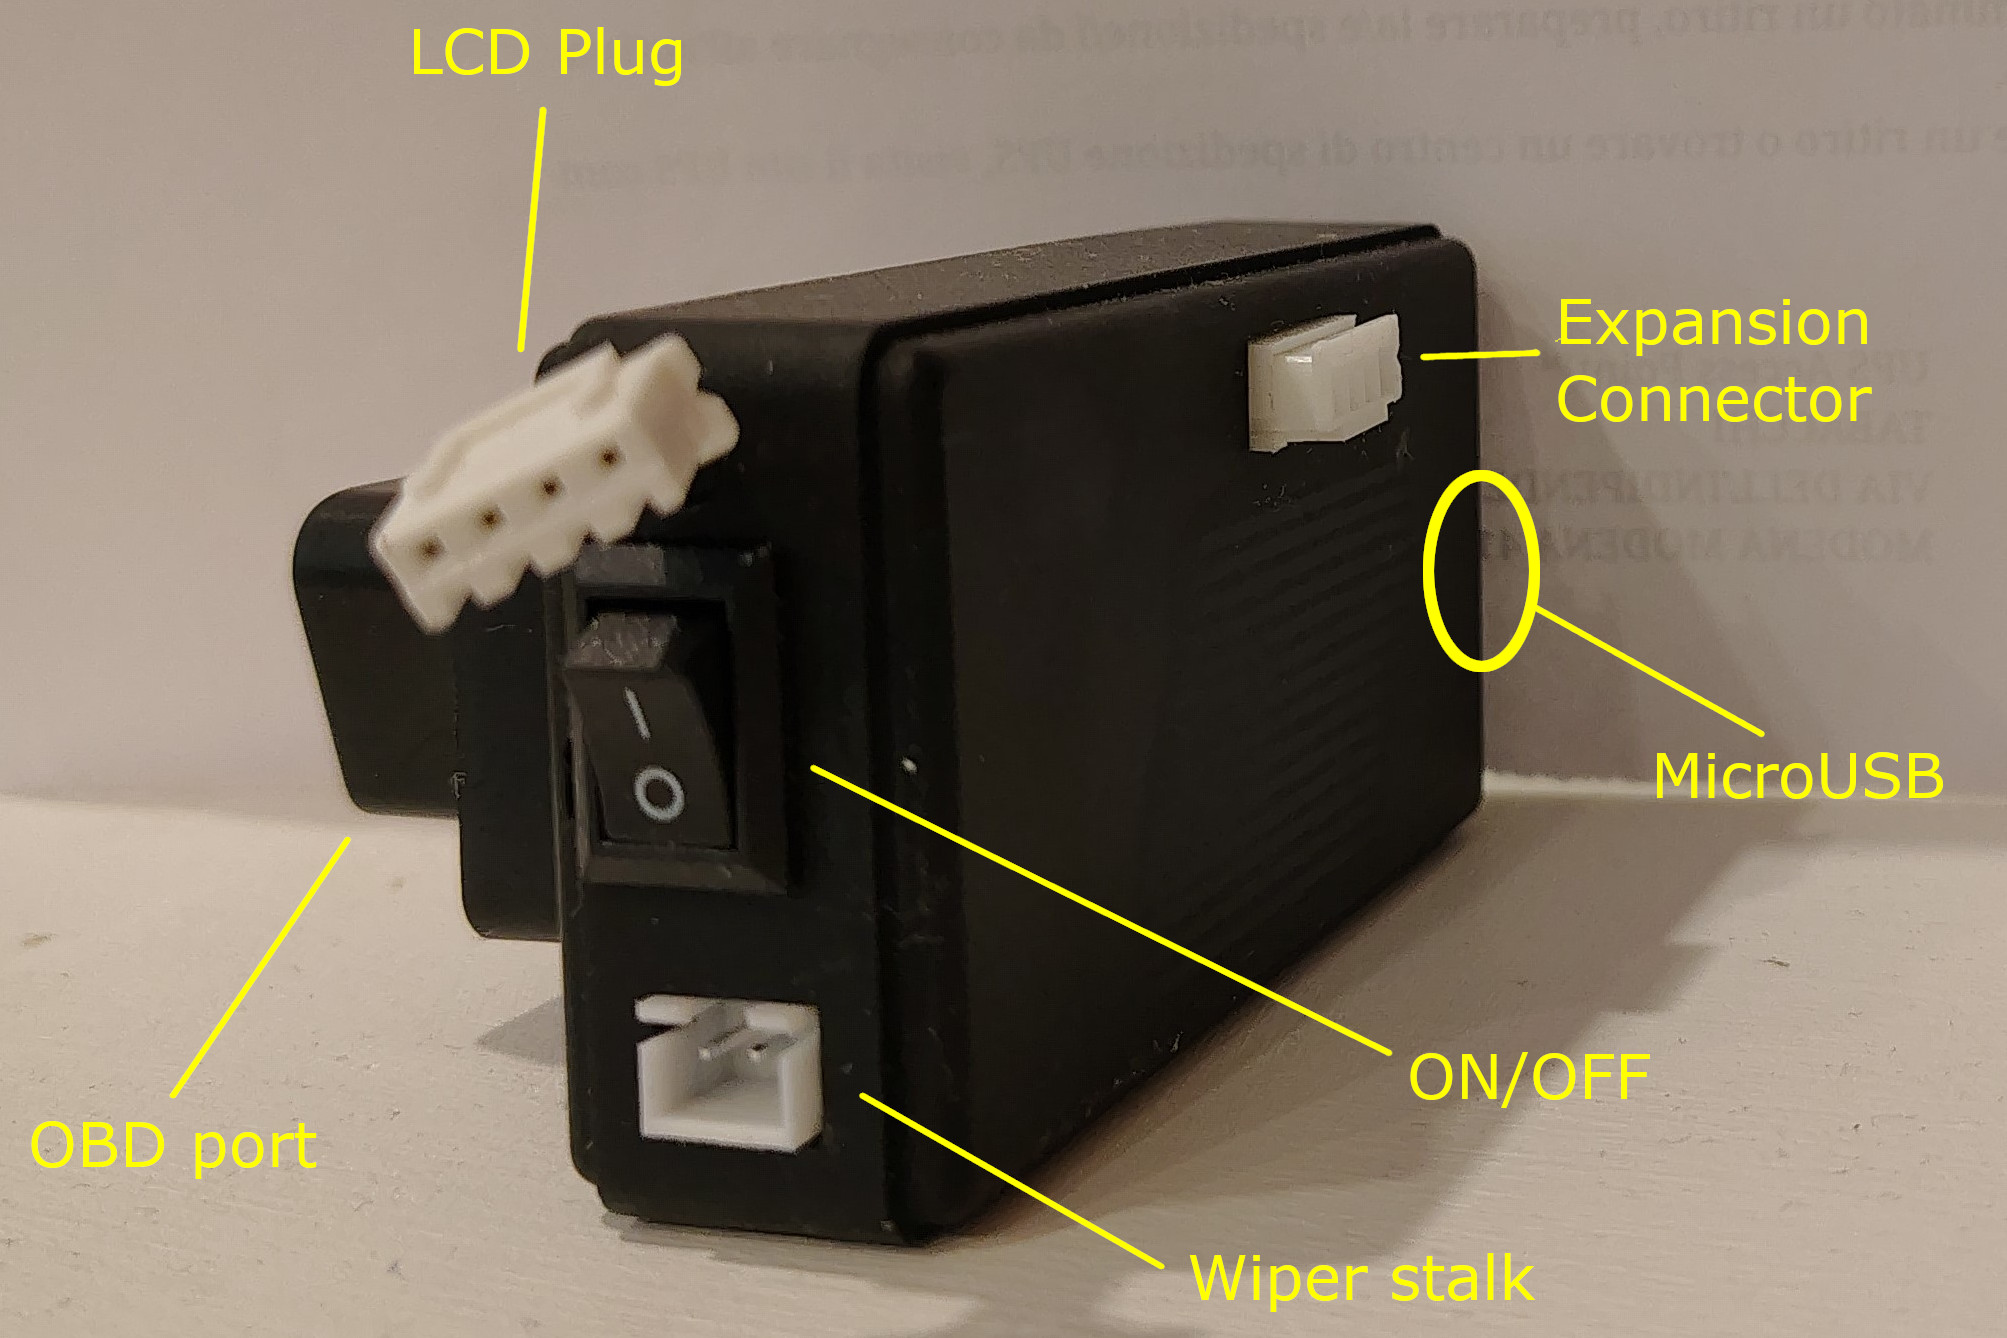
\includegraphics[width=0.75\textwidth]{figures/black_box.jpg}
    \caption{The black box}
\end{figure}

\subsection{The Expansion Connector}

If you would like to customize more your ToM+ you can easily do this using the connector
shown in the image here. In fact it gives an additional 5V power supply coming from
VCC (ex red cable) and the GND (ex black cable), so that you can power an external LED, a
small buzzer or whatever you prefer. The other two cables are General Input Output
Pins, PIN1 (ex yellow) and PIN2 (ex blue). They can have either input or output functions, depending on what you will choose on the \textit{“Expansion page”} of ToM \textbf{web server}. In this latest version of the device, the expansion connector is embedded in the black box (without colored cables) but the pinout remains the same.
Remember to remove the protective cover before using it and to use an input voltage of \textbf{maximum 3,3V}. For higher
voltage provide a proper resistor divider.

\begin{figure}[H]
    \centering
    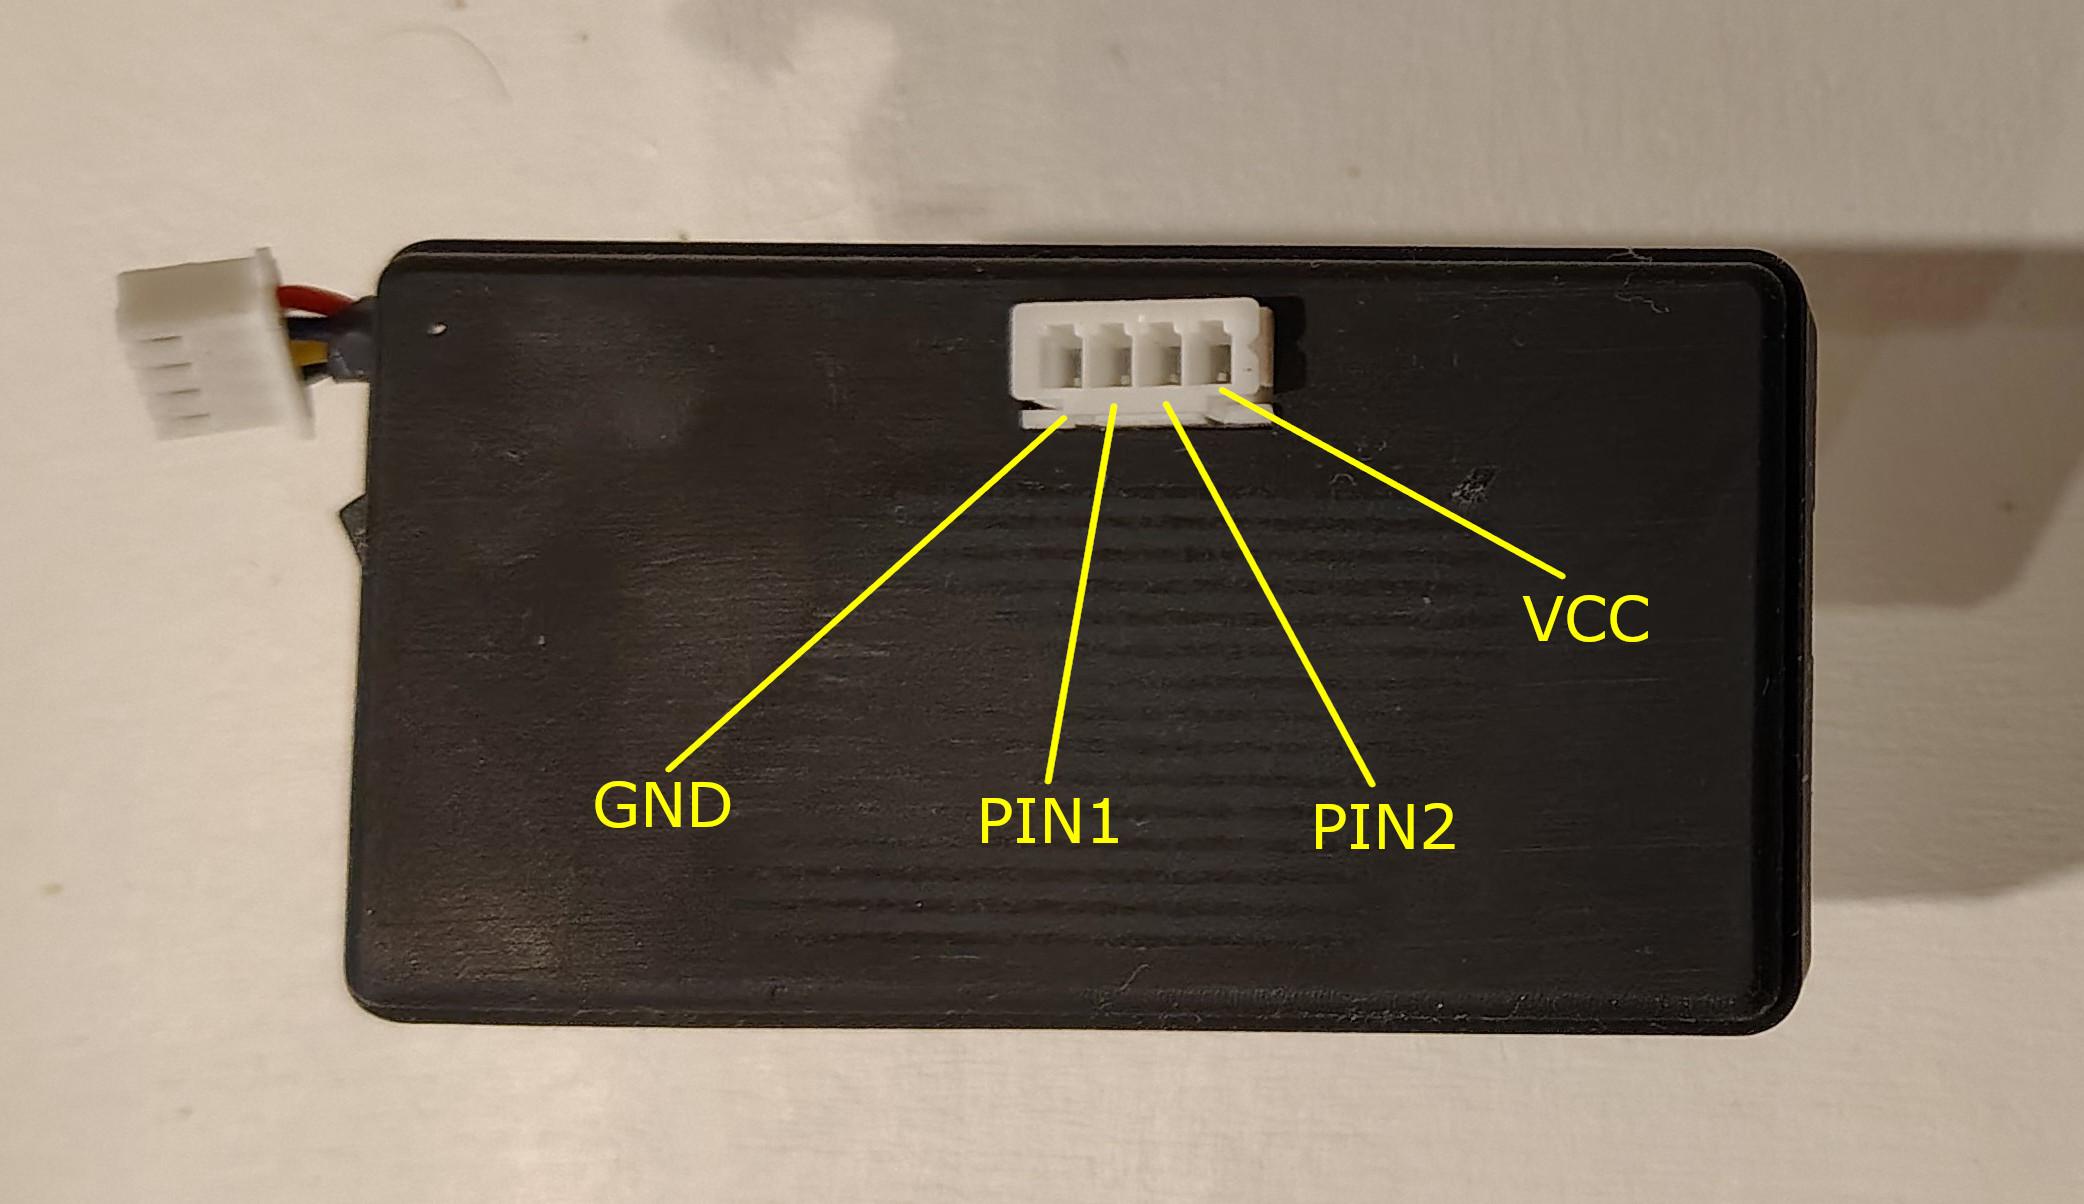
\includegraphics[width=0.7\textwidth]{figures/expansion_bb.jpg}
    \caption{Expansion connector}
    \label{fig:expansion_pinout}
\end{figure}

\subsection{The LCD Display and stand}

The resistive touch LCD display is embedded in a 3D printed stand that clips on the original dashboard. If requested, you can also have a 3D standalone support to mount the display on the glovebox as the standard ToM. In that way, you can have a 2 in 1 device that can be both clip-on or standalone as you wish. A microSD slot is accessible for firmware updates.

\begin{figure}[H]
    \centering
    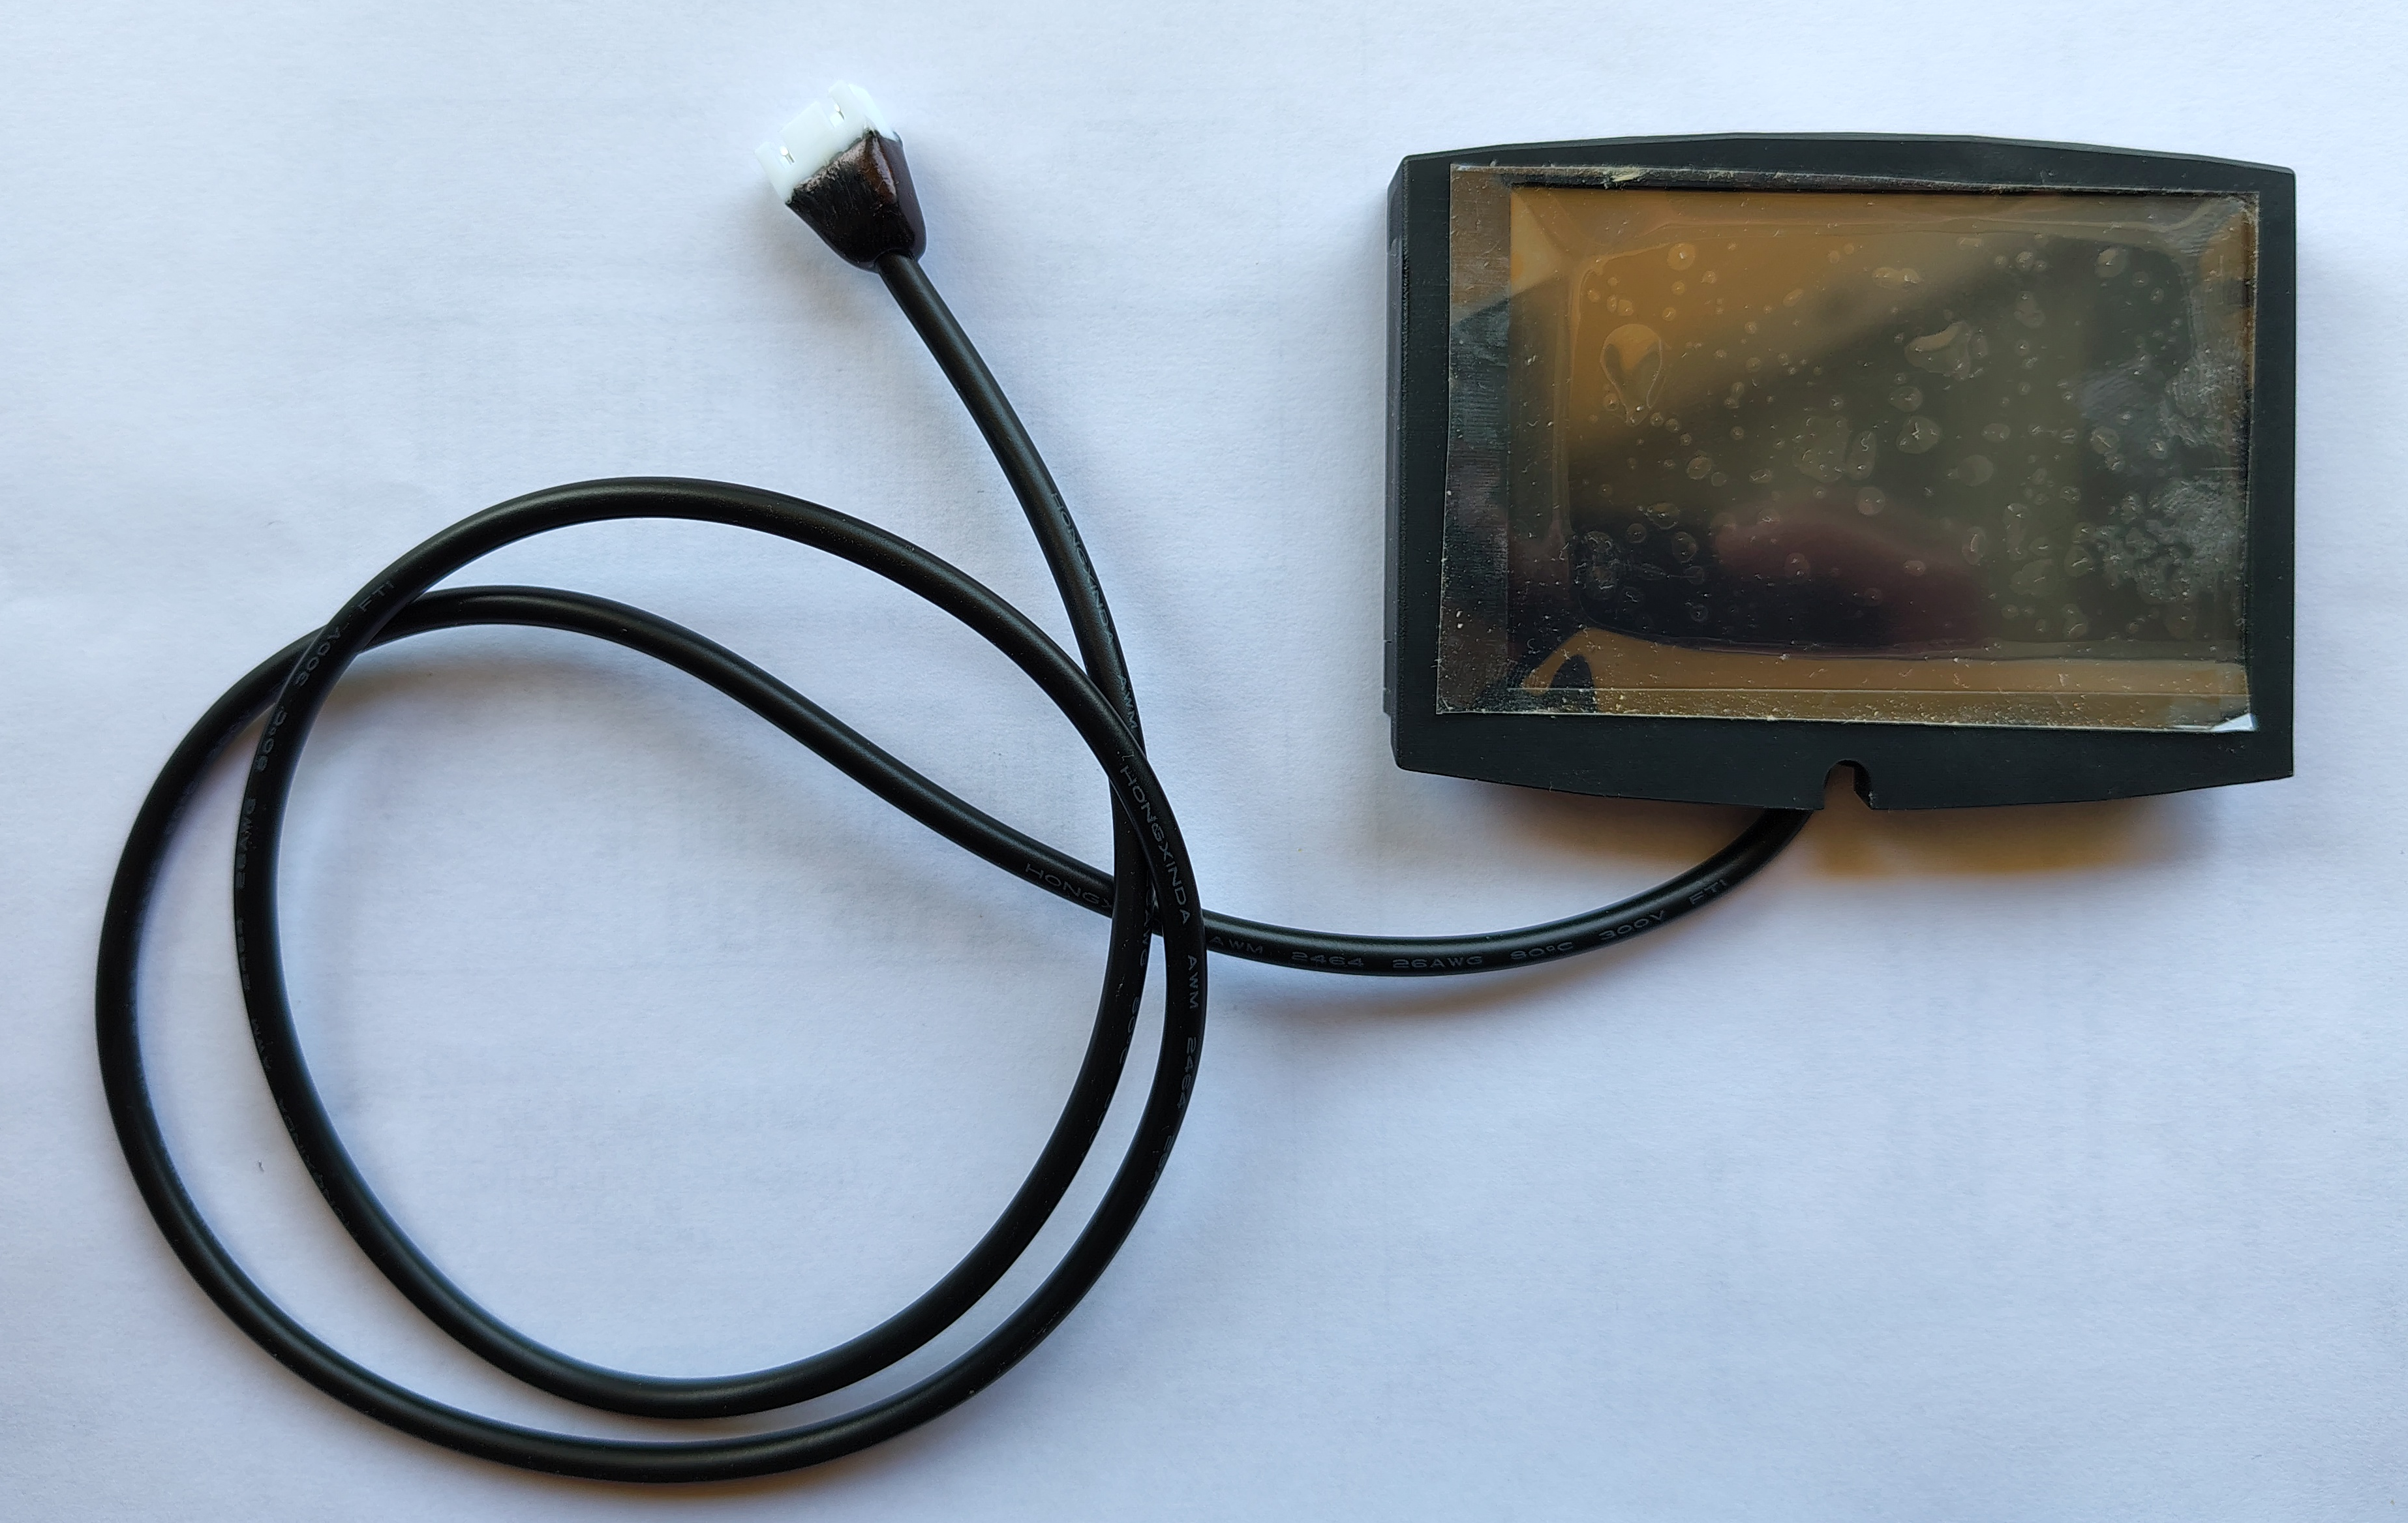
\includegraphics[width=0.8\textwidth]{figures/display.png}
    \caption{LCD display clip-on}
\end{figure}

The display, provided with a protective film, as visible in the images, can be put into the 3D container to have an adjustable stand that you can put wherever you like.

\begin{figure}[H]
    \centering
    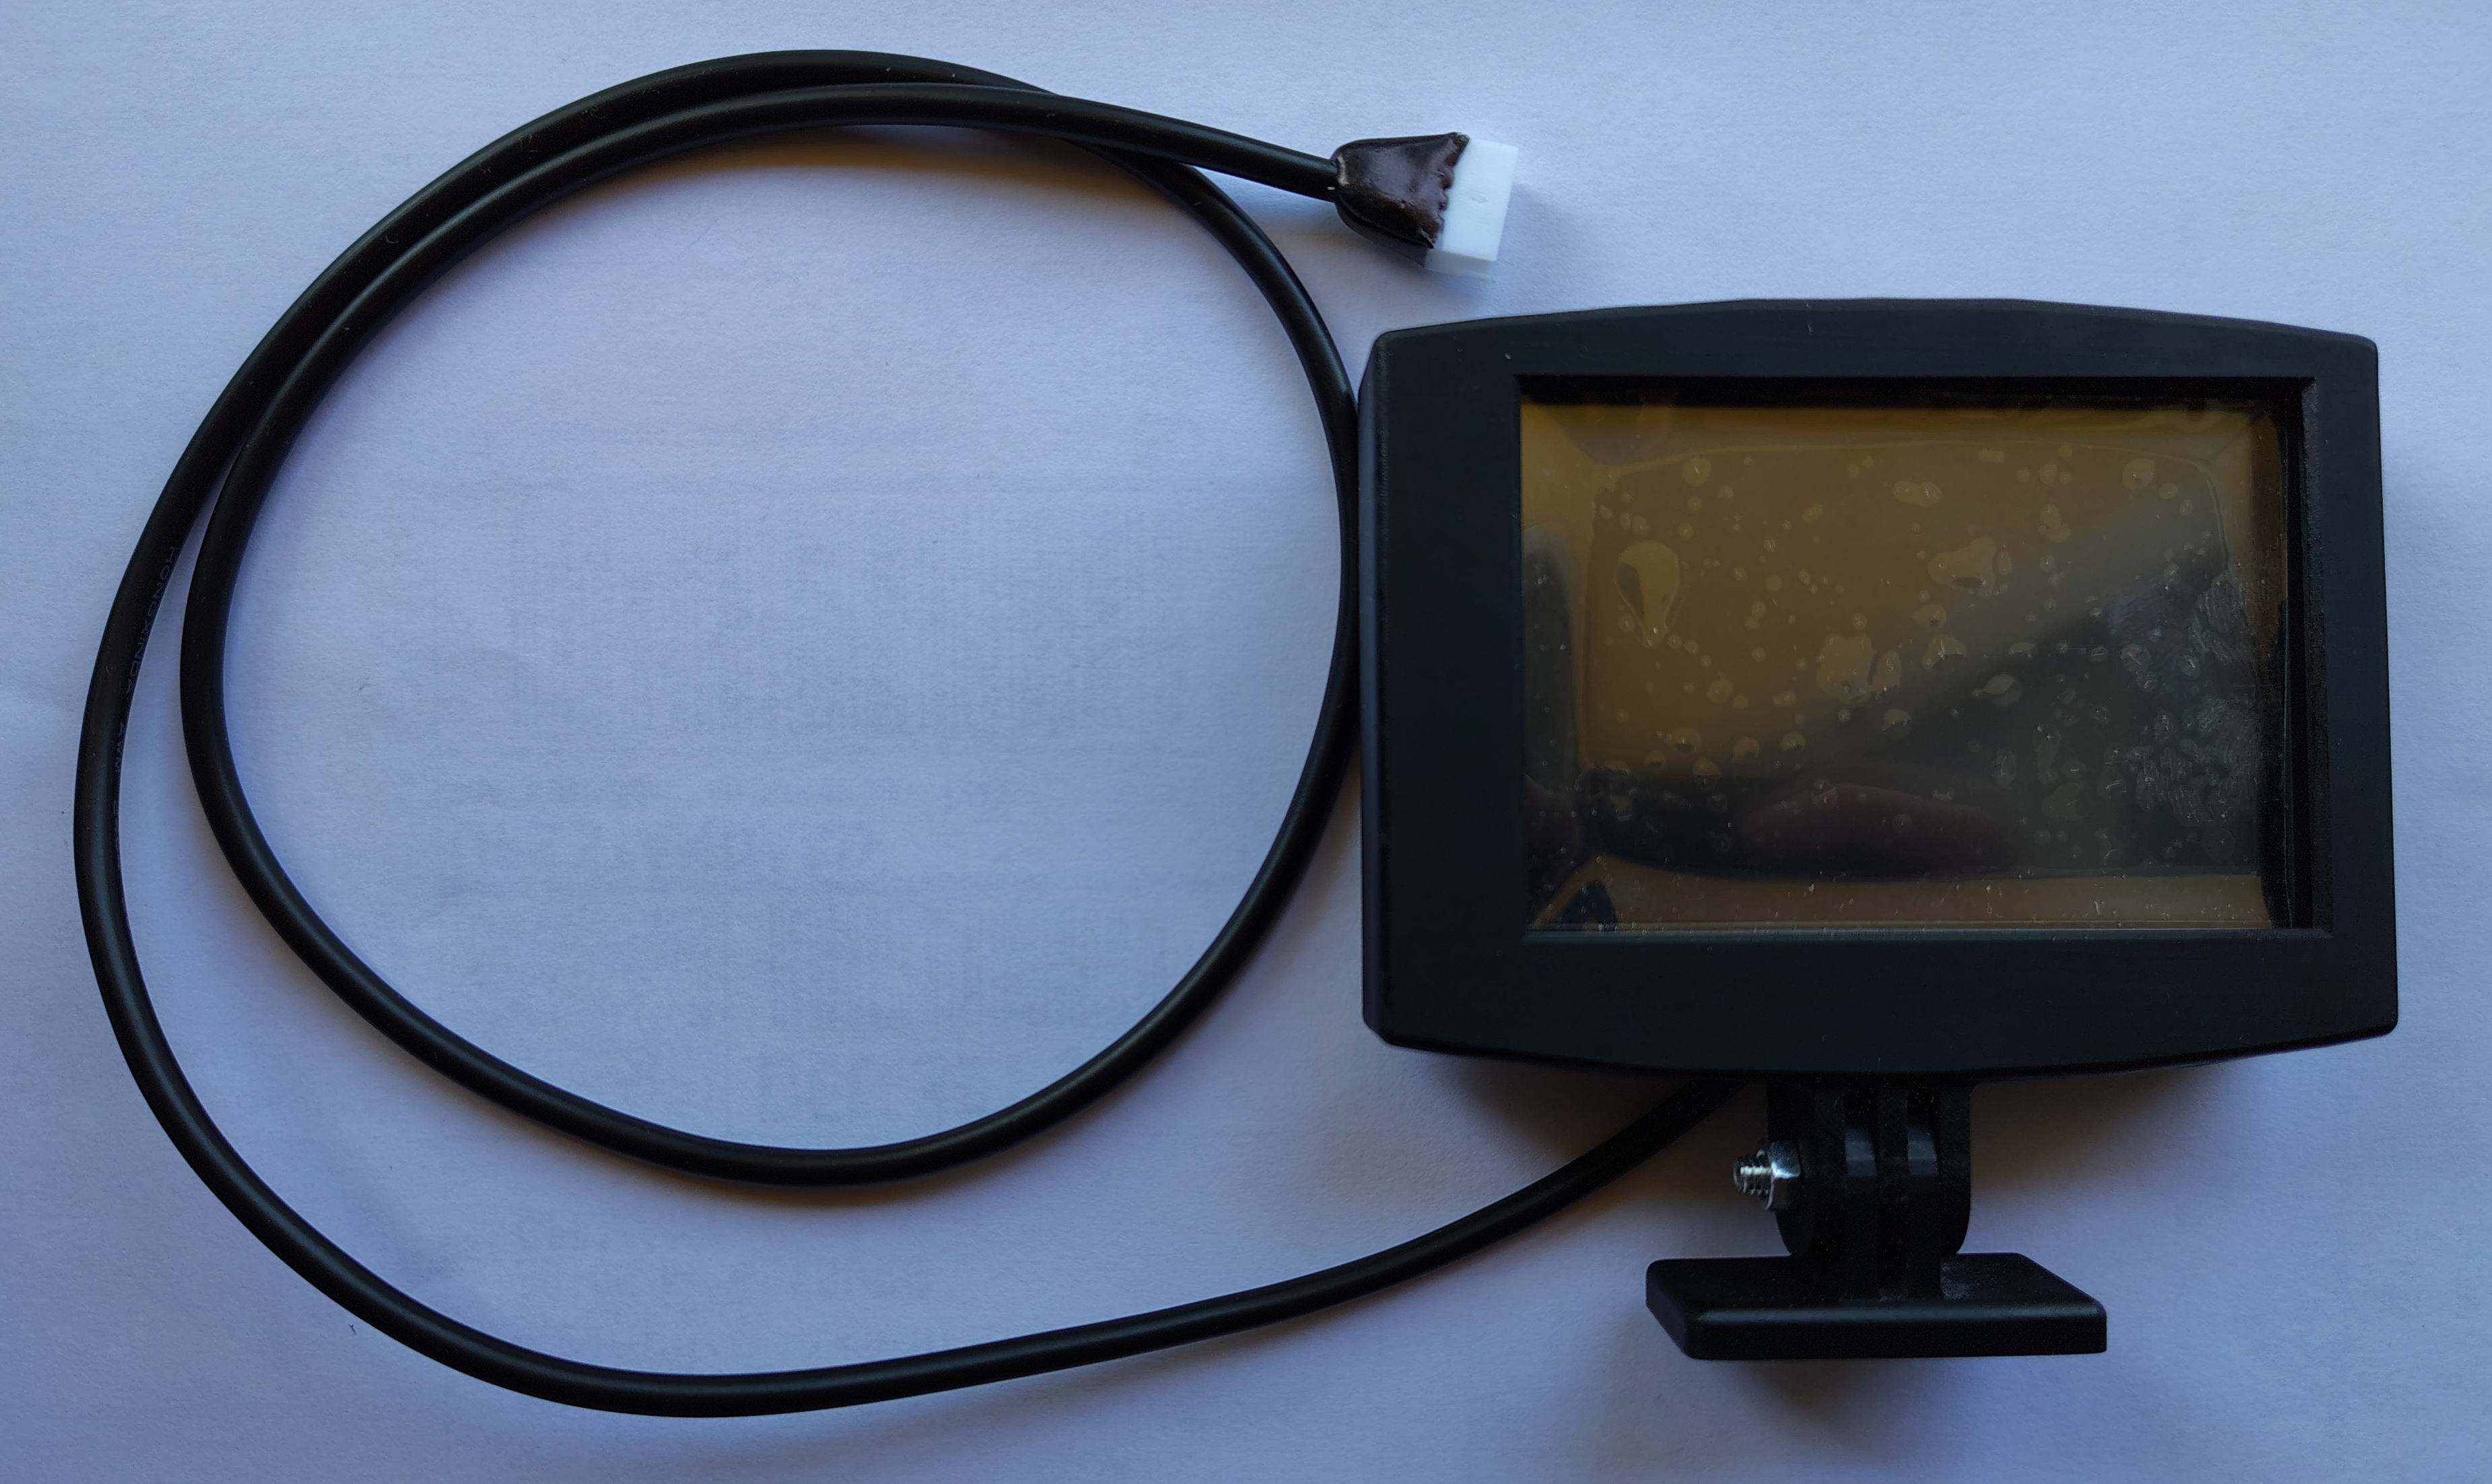
\includegraphics[width=0.8\textwidth]{figures/3d_stand_wdisplay.png}
    \caption{LCD display standalone}
\end{figure}

When inside the standalone version, you can fix it with the cover and the screws that you can find in the packet along with the 3D foldable stand, as shown in the images below.

\begin{figure}[H]
    \centering
    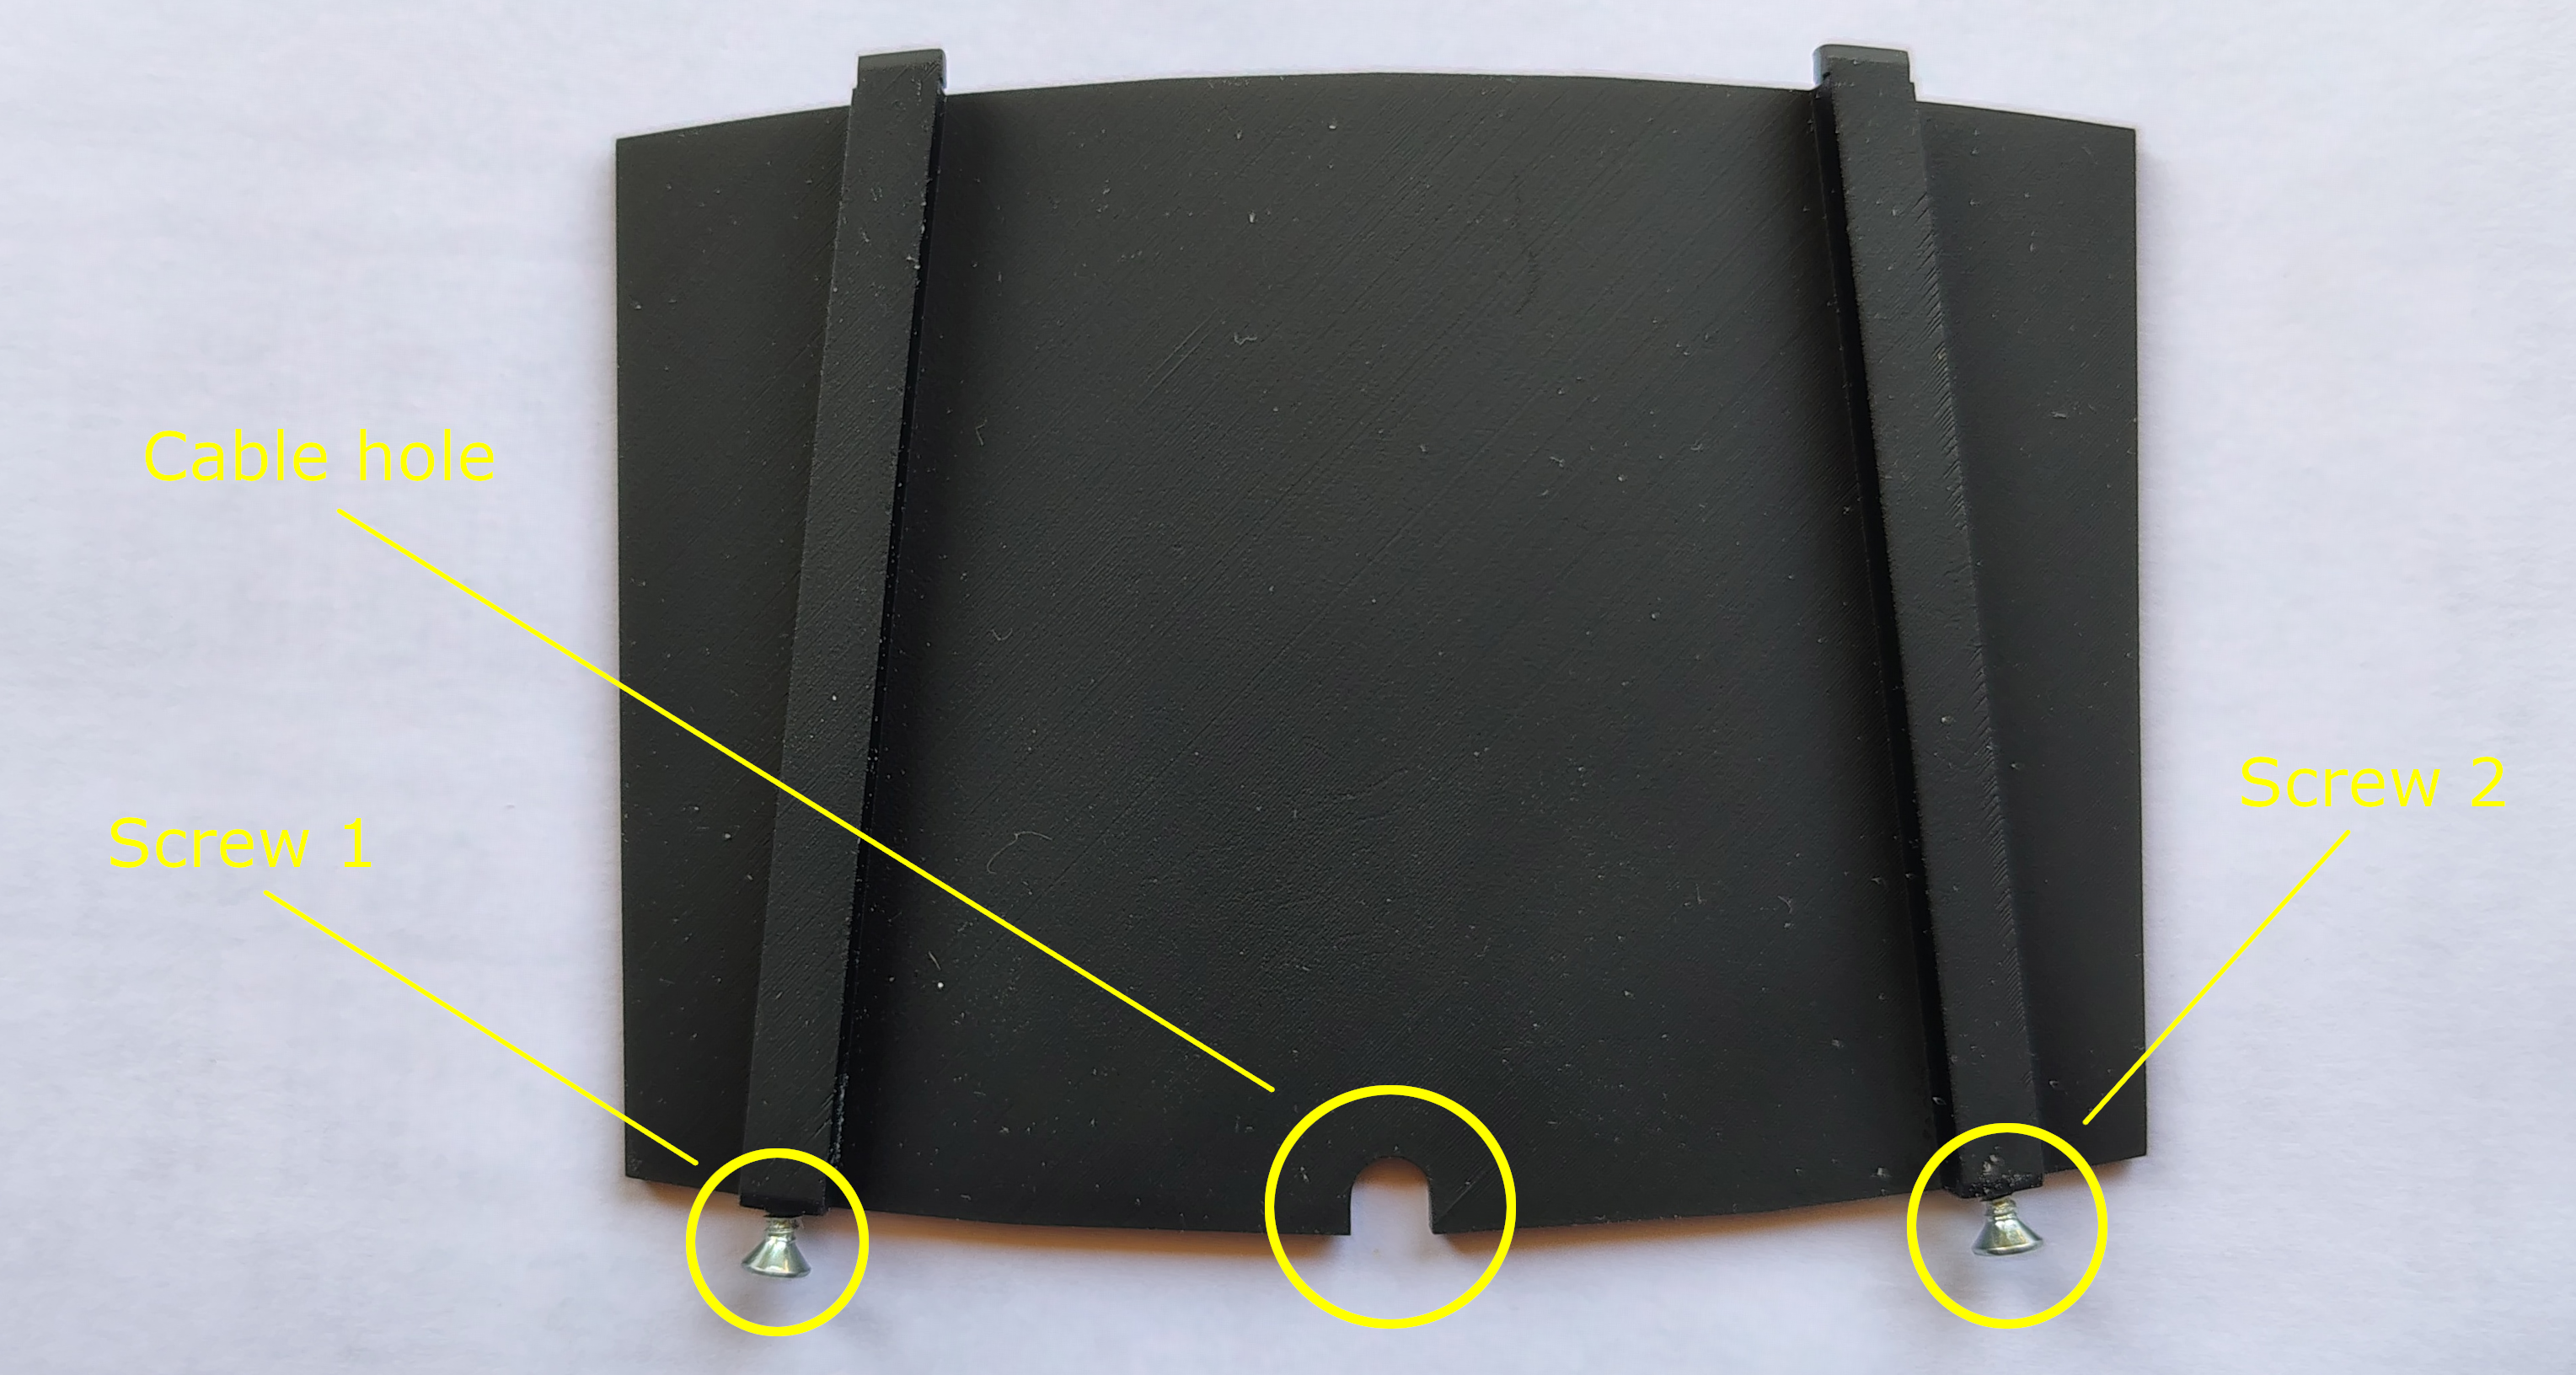
\includegraphics[width=0.8\textwidth]{figures/back_cover.png}
    \caption{LCD cover provided}\label{fig:back_cover}
\end{figure}

The 3D stand also has holes on the base if you want to screw it on the glovebox. The other holes on the frame are made for screwing the back cover to keep the display in place when inside.

\begin{figure}[H]
    \centering
    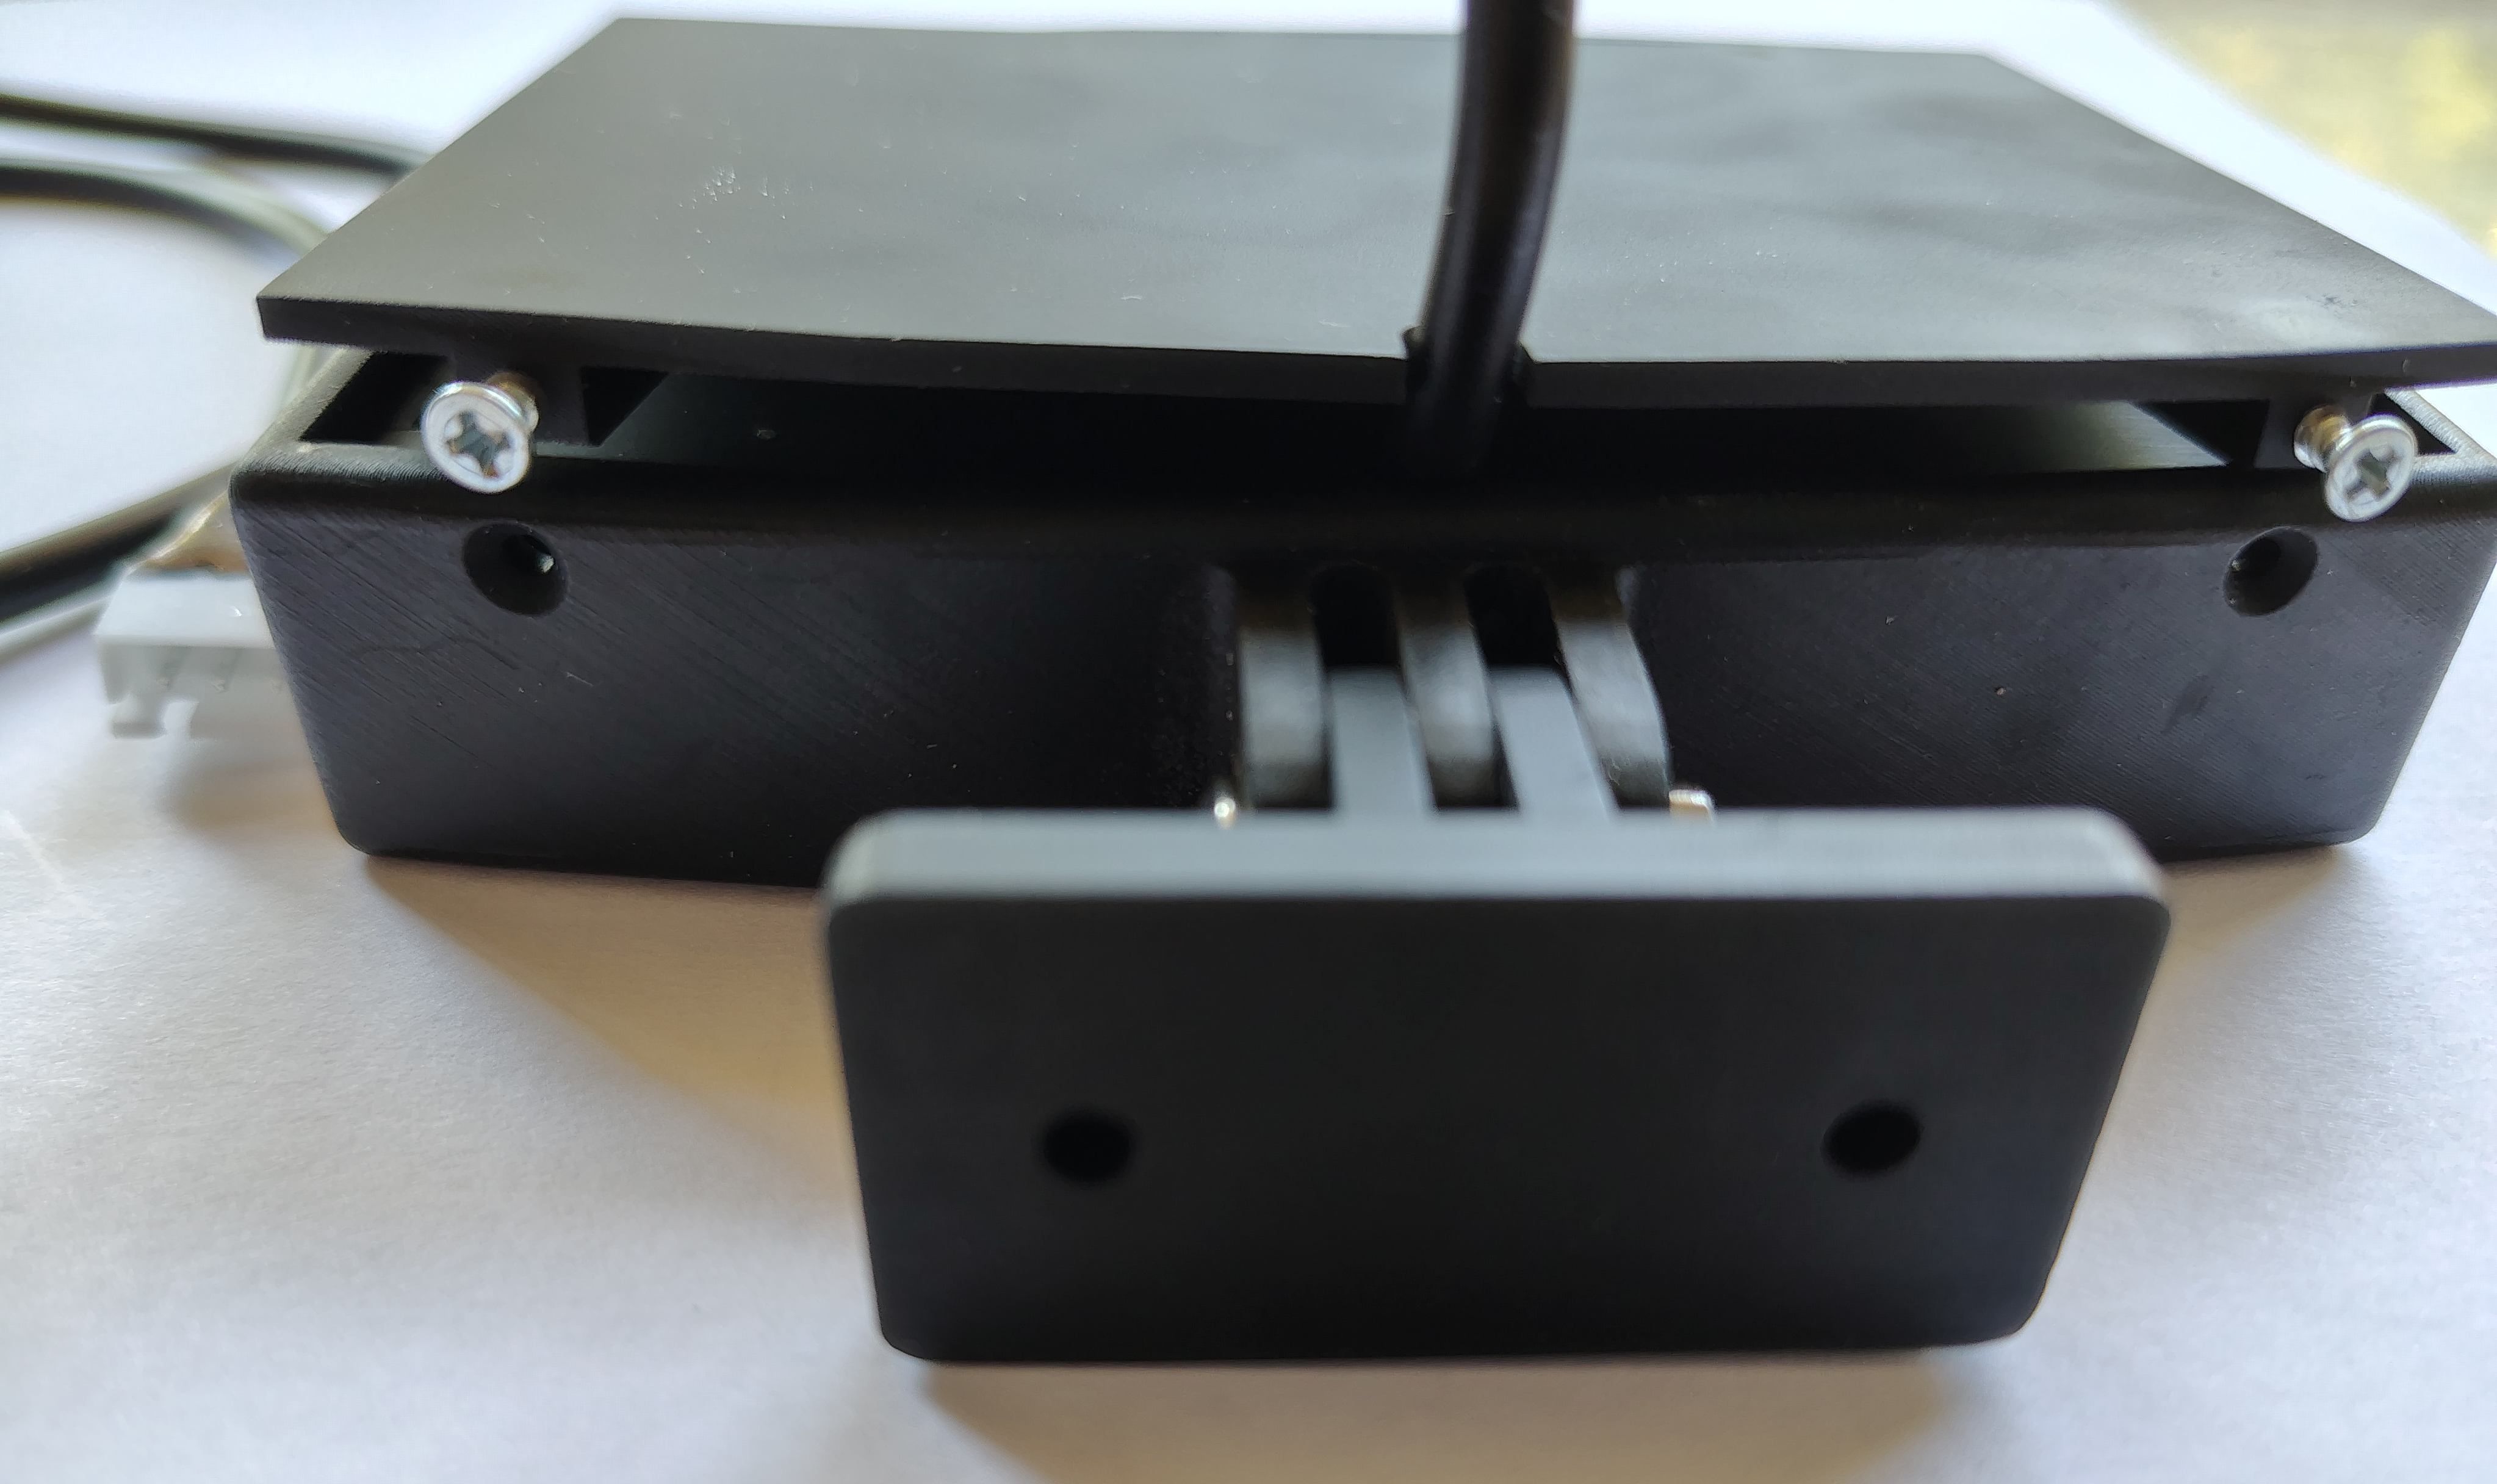
\includegraphics[width=0.8\textwidth]{figures/bottom_cover_screwholes.png}
    \caption{LCD cover screw fixing}\label{fig:bottom_cover_screwholes}
\end{figure}

\subsection{Additional Useful Components}

The package includes a cable tie to fix the 3D printed stand for the button to the right wiper stalk (included as well). In addition, there is a bonus sticker if you want to support the project by sticking it somewhere on your Twizy.

\begin{figure}[H]
    \centering
    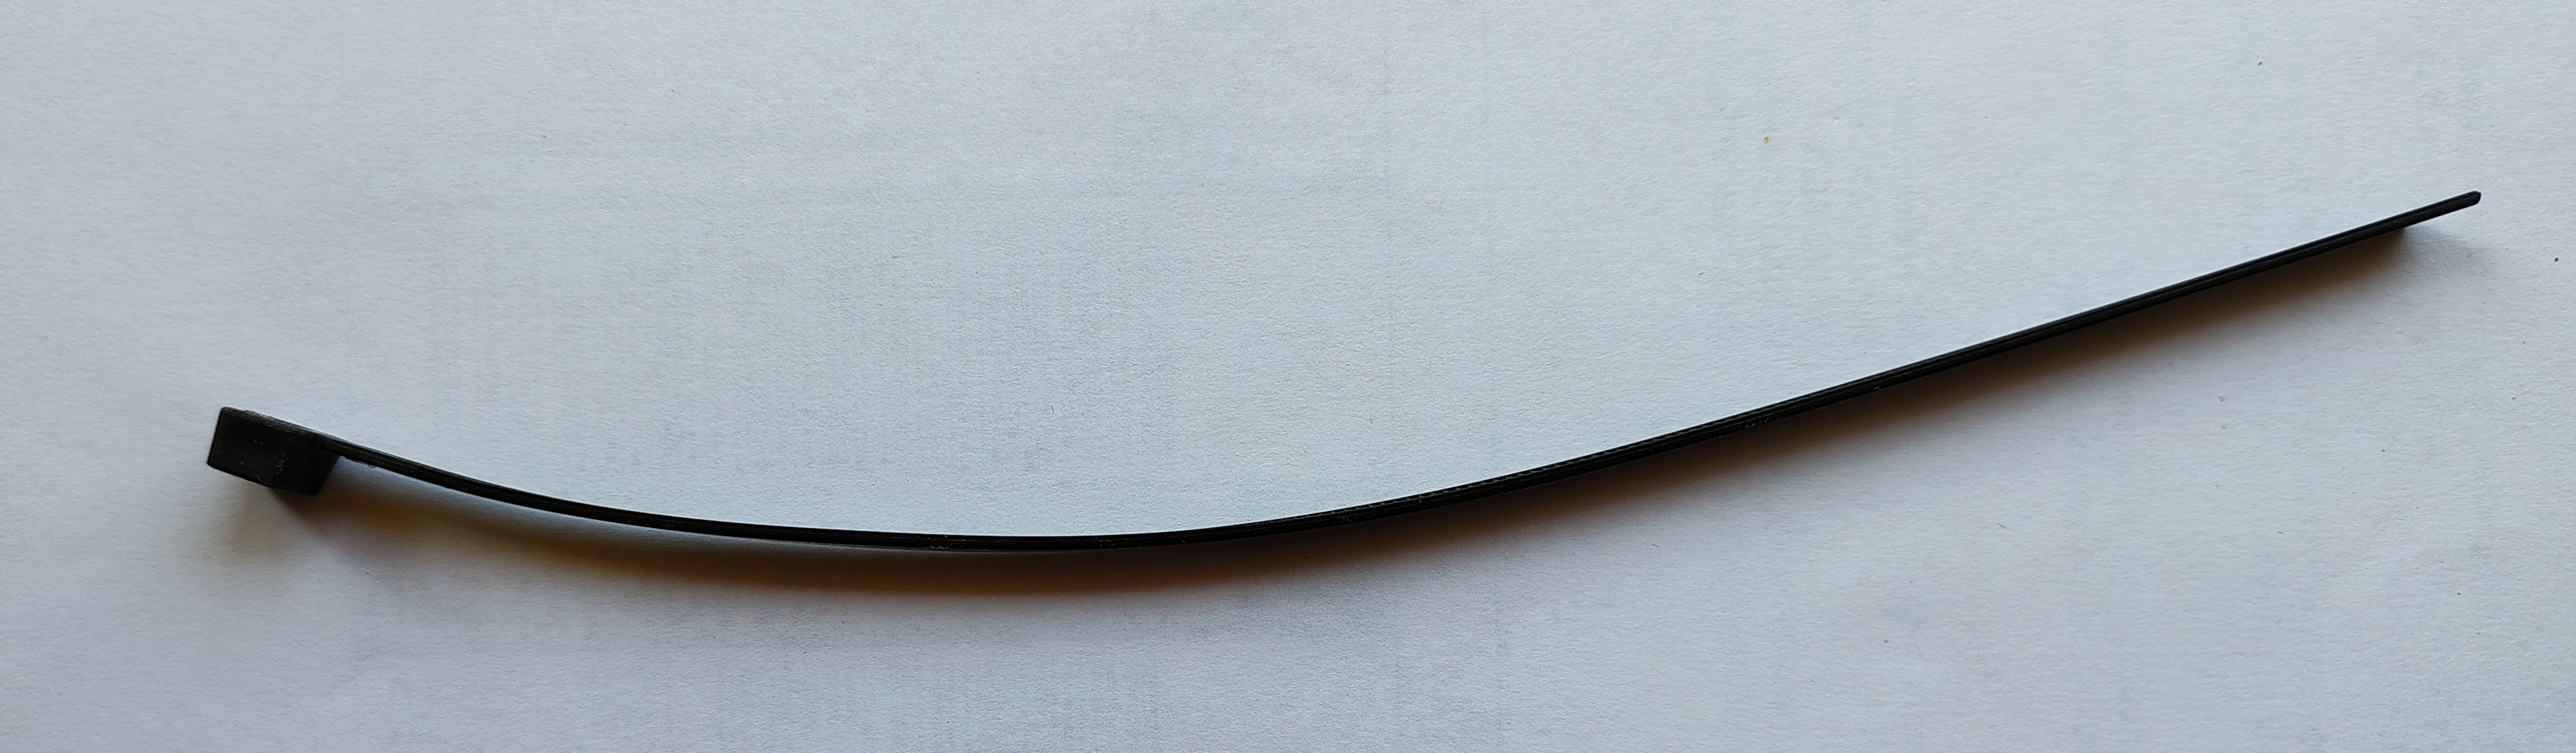
\includegraphics[width=0.8\textwidth]{figures/cable_tie.jpg}
    \caption{Cable tie}
\end{figure}

\begin{figure}[H]
    \centering
    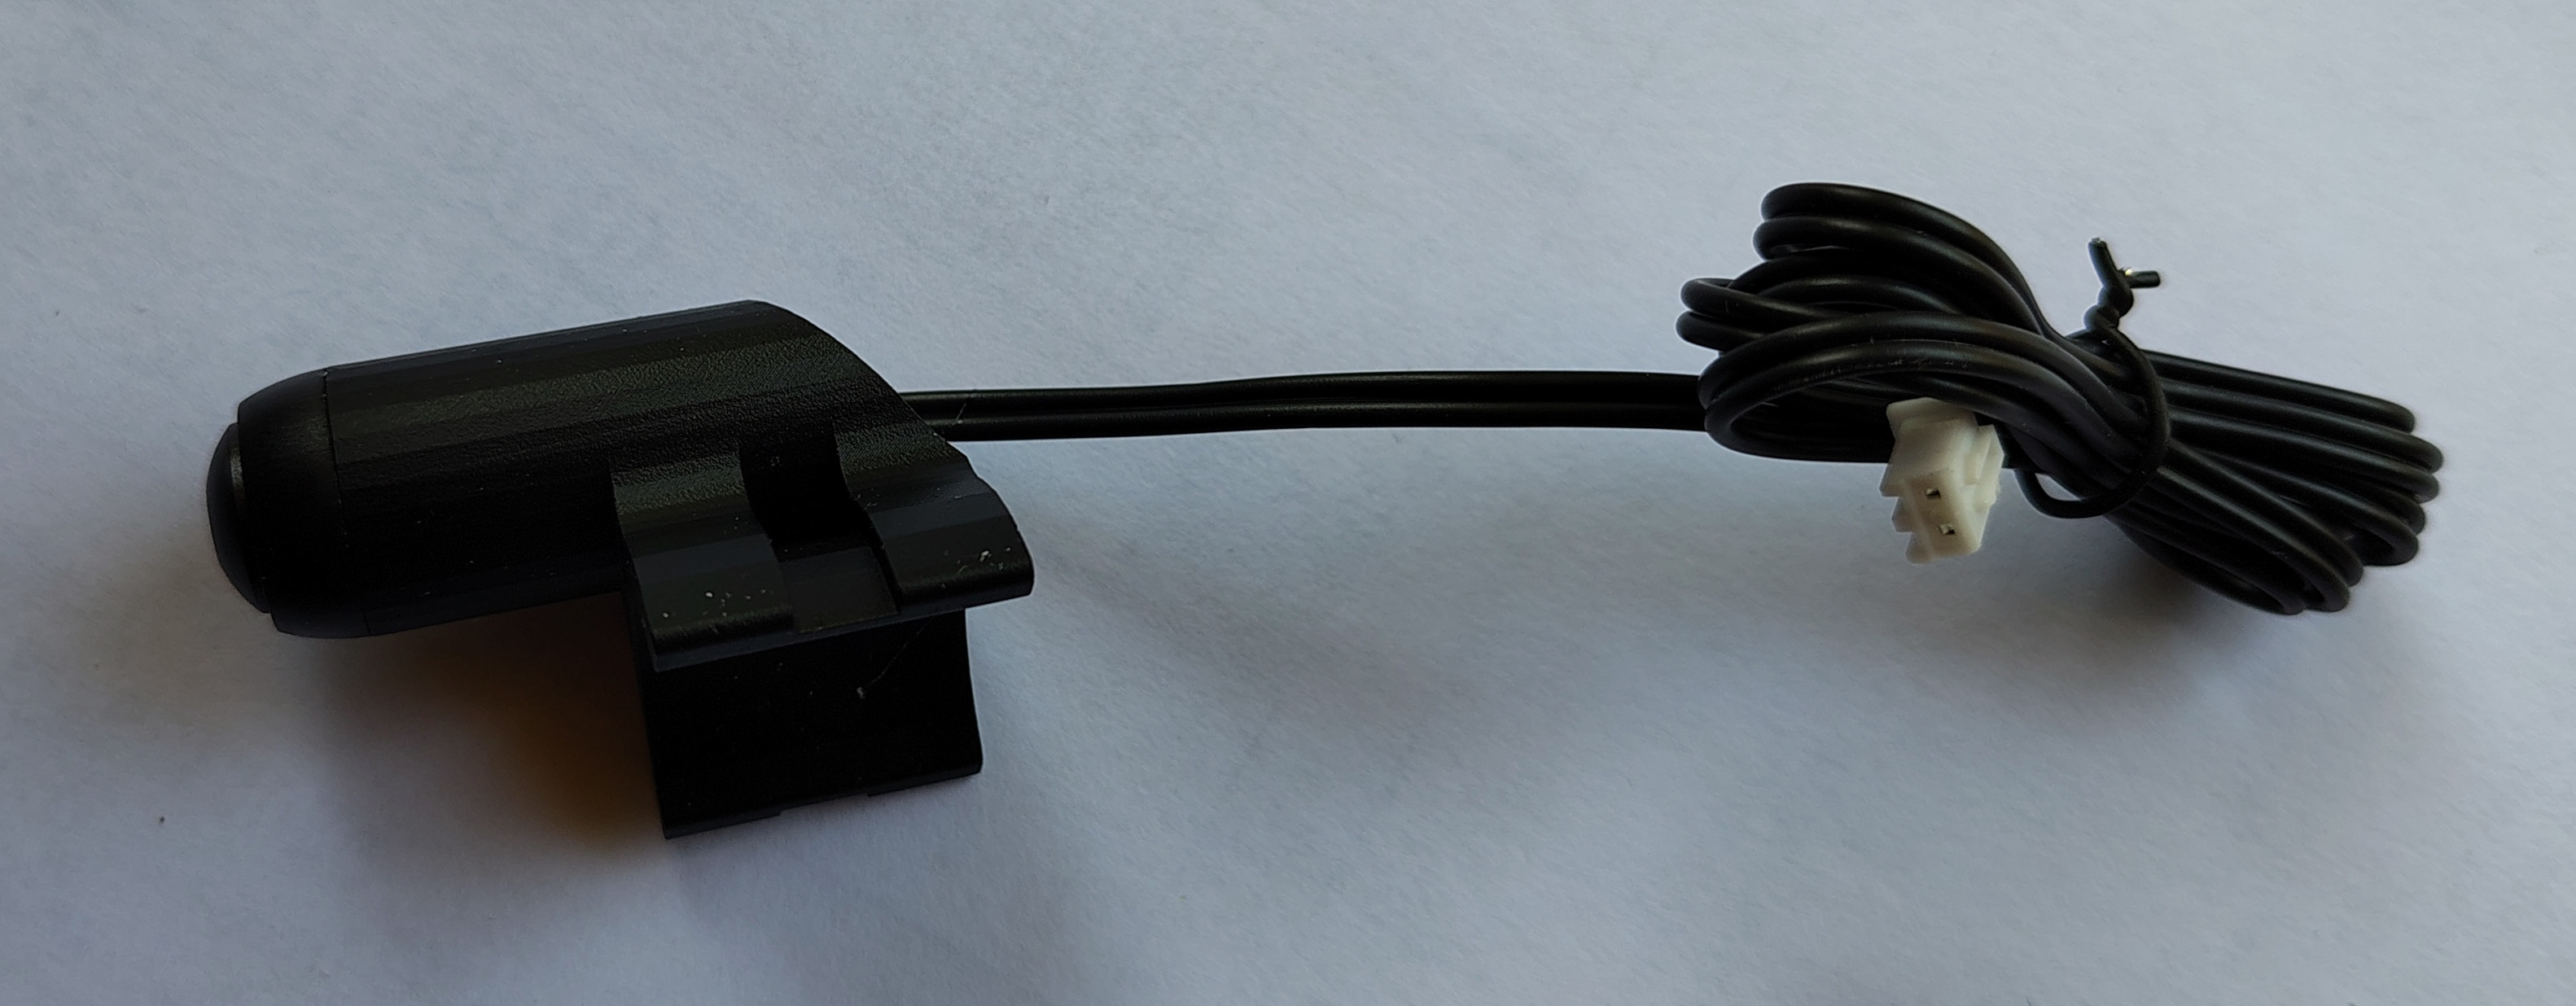
\includegraphics[width=0.8\textwidth]{figures/wiper_stalk_button.jpg}
    \caption{3D printed button for wiper stalk}\label{fig:wiper_stalk_button}
\end{figure}

\begin{figure}[H]
    \centering
    
\includegraphics[width=0.8\textwidth]{figures/sticker.png}
    \caption{ToM sticker}
\end{figure}